\chapter{Distribution}
\label{cha:distribution}
\headerblock{
  \headerquote{If we expect concurrent programming to become
mainstream, and if we demand reliability and predictability from programs, we must discard threads as
a programming model. We can construct concurrent
programming models that are much more predictable
and understandable than threads based on a simple principle: Deterministic ends should be accomplished with
deterministic means.}{Edward A. Lee~\cite{lee2006problem}}
}

This section considers the problem of automatic distribution of streaming operators.
Rather than use the structured representation of \Cref{cha:composition},
distribution requires a more low-level representation because it requires knowing how an operator can be parallelized.
In the chapter, we will define a programming model over streams called \emph{dependency guided synchronization} and show how it can be used to parallelize stream operators automatically.
The material in this section was originally published in~\citeMain{ppopp22}.

Tying this into determinism are two fundamentally important theorems to the chapter: \Cref{dgs:thm:consistency-implies-determinism} which states that for the programming model, \emph{consistency implies determinism}; and \Cref{dgs:theorem:correctness}, which states that the end-to-end system is correct and in particular, distribution is semantics-preserving.

\section{Motivation}

The success of stream processing APIs based on the dataflow model can be attributed to their ability to simplify the task of parallel programming. To accomplish this (as described in \Cref{bg:autoparallelization}), most APIs expose a simple but effective model of data-parallelism called \emph{sharding} (\emph{auto-parallelizaiton}), in which
nodes in the dataflow graph are replicated into many parallel instances, each of which
will process a different partition of the input events.
However, while sharding is intuitive for programmers, it also implicitly limits the scope of parallel patterns that
can be expressed. Specifically, it prevents arbitrary
\emph{synchronization across parallel instances}
since it disallows communication between them.
This is limiting in modern applications such as video processing \cite{chienchun2018videoedge} and distributed machine learning \cite{otey2006fast}, since they require both synchronization between nodes and high throughput and could therefore benefit from parallelization.
Further evidence that sharding is limiting in practice
can be found in a collection of feature requests in state-of-the-art stream processing systems~\cite{dgs-feature-request1,dgs-feature-request2,dgs-feature-request3}, asking either for state management that goes beyond replication or for some form of communication between shards.
To address these needs, system developers have introduced
extensions to the dataflow model to enable specific use cases such as  \emph{message broadcasting} and \emph{iterative dataflows}.
However, existing solutions do not generalize,
as we demonstrate experimentally in \Cref{dgs:ssec:eval-existing-implementations}.
For the remainder of applications, users are left with two unsatisfying solutions: either ignore parallelization potential, implementing their application
with limited parallelism; or circumvent the stream processing APIs using low-level external mechanisms to achieve synchronization between parallel instances.

For example, consider a fraud detection application where the input is a distributed set of streams of bank transaction events. Suppose we want to build an unsupervised online machine learning model over these events which classifies events as fraudulent based on a combination of \emph{local} (stream-specific) and \emph{global} (across-streams) statistical summaries.
The problem with the traditional approach is that when classifying a new event, we need access to both the local and the global summaries; but this cannot be achieved using sharding since by default shards do not have access to a global summary.
One extension to the dataflow model, implemented in some systems~\cite{Flink,Timely} is the \emph{broadcast} pattern, which allows the operator computing the global summary to broadcast to all other nodes.
However, broadcasting is restricted since it does not allow bidirectional communication;
the global summary needs to be both broadcast to all shards, but also updated by all shards.
Cyclic dataflows are another partial solution, but do not always solve the problem, as we show in \Cref{dgs:ssec:eval-existing-implementations}.
In practice, applications like this one with complex synchronization requirements opt to  manually
implement the required synchronization using
external mechanisms (e.g. querying a separate a key-value store with strong consistency guarantees). This is error prone and, more importantly, violates the requirements of many streaming APIs that operators need to be effect-free so that the underlying system can provide exactly-once execution guarantees in the presence of faults.

\section{Contributions}

To address the need to combine parallelism with synchronization, we make two contributions. First, we propose \emph{synchronization plans}, a tree-based execution model which is a restricted form of communicating sequential processes~\cite{hoare1978communicating}.
Synchronization plans are hierarchical structures that represent concurrent computation in which parallel nodes are not completely independent, but communicate with their ancestors on special synchronizing events.
While this solves the problem of being able to express synchronizing parallel computations, we still need a streaming API which exposes such parallelism implicitly rather than explicitly.
For this purpose, we propose \emph{dependency-guided synchronization} (DGS), a parallel programming model which can be mapped automatically to synchronization plans.

A DGS program consists of three components. First, the user provides a \emph{sequential implementation} of the computation; this serves to define the semantics of what they want to compute assuming the input is processed as a sequence of events.
Second, the user indicates which input events can be processed in parallel and which require synchronization by providing a \emph{dependence relation} on input events.
This relation induces a partial order on the input stream.
For example, if events can be processed completely in parallel without any synchronization, then all input events can be specified to be independent.
Third, the user provides a mechanism for parallelizing state when the input stream contains independent events: \emph{parallelization primitives} called \emph{fork} and \emph{join}. This model is inspired by classical parallel programming, but has streaming-specific semantics which describes how a partially ordered input stream is decomposed for parallel processing.

Given a DGS program, the main technical challenge is to generate
a synchronization plan, which corresponds to a concrete implementation, that is both \emph{correct} and \emph{efficient}. More precisely, the challenge lies in ensuring that a derived implementation correctly enforces the specified input dependence relation. To achieve correctness, we formalize: (i) a set of conditions that ensure that a program is consistent, and (ii) a notion of $P$-\emph{valid} synchronization plans, i.e., plans that are well-typed with respect to a given program $P$.
To achieve efficiency, we design the framework so that correctness is independent of \emph{which} synchronization plan is chosen---as long as it is $P$-valid.
The idea of this separation is to enable future work on optimized query execution, in which an optimizing component searches for an efficient synchronization plan maximizing a desired cost metric without jeopardizing correctness.
We tie everything together by proving that the end-to-end system is correct,
that is, any concrete implementation that corresponds to an $P$-valid plan is equivalent to a program $P$ that satisfies the consistency conditions.

In order to evaluate DGS, we perform a set of experiments to investigate the data parallelism limitations of Flink~\cite{Flink2015}---a representative high-performance stream processing system---and
Timely Dataflow~\cite{Naiad2013}---a representative system with iterative computation.
We show that these limits can be partly overcome by manually implementing synchronization. However, this comes at a cost: the code has to be specialized
to the number of parallel nodes and similar implementation details, forcing
the user to sacrifice the desirable benefit of \emph{platform independence}.
We then develop Flumina, an end-to-end prototype that implements DGS in Erlang~\cite{armstrong1993erlang}, and show that it can automatically produce scalable implementations (through generating synchronization plans from the program) independent of parallelism.
In the extended version of the paper~\cite{flumina-arxiv},
we also evaluate programmability via two real-world case studies.
In particular,
we demonstrate that the effort required---as measured by lines of code---to achieve parallelism is minimal compared to the sequential implementation.

In summary, we make the following contributions:
\begin{itemize}
\item
\emph{DGS:} a novel programming model for parallel streaming computations that require synchronization, which allows viewing input streams as partially ordered sets of events. (\Cref{dgs:sec:prog-model})
\item
\emph{Synchronization plans:} a tree-based execution model for parallel streaming computations that require synchronization, a framework for generating a synchronization plan given a DGS program, a prototype implementation, and an end-to-end proof of correctness.
(\Cref{dgs:sec:dist-impl})
\item
An evaluation that demonstrates: (i) the throughput limits of automatically scaling computations on examples which require synchronization in Flink and Timely; (ii) the throughput and scalability benefits achieved by synchronization plans over such automatically scaling computations; and (iii) the programmability benefits of DGS for synchronization-centered applications
(\Cref{dgs:sec:evaluation}).
\end{itemize}

Flumina, our implementation of DGS, is open-source and available
\githubref{https://github.com/angelhof/flumina}{on GitHub}.

% \section{Motivating Examples}
% \label{dgs:ssec:motivating-application}
%
% \paragraph{Fraud detection}
% Suppose there are two types of input events: bank transactions and fraud detection rules
% that are used to flag some transactions as fraudulent. Bank
% transactions are continuously input in the system with high rate while new
% fraud detection rules arrive infrequently. An example of a new rule would
% be the addition of a specific account to an index of suspicious accounts.
% There is no way to partition inputs while
% avoiding cross-partition dependencies since all events (both
% transactions and rules) depend on previous rule events. Still, if the
% rate of bank transaction events becomes a bottleneck (and fraud
% detection rule events happen rarely) it would be beneficial to
% parallelize the processing of bank transaction events.
%
% One of the solutions that has been used to achieve data parallelism in
% such computations involves extending the dataflow model with a
% \emph{broadcast} pattern that allows sending some input events to \emph{all}
% parallel shards (and partitioning the rest of the events as usual). An
% example execution of the above computation that utilized the broadcast
% pattern is shown in \Cref{dgs:fig:broadcast-dependencies-vis}. By
% broadcasting the fraud detection rule events, a parallel implementation
% is achieved without requiring cross-instance communication between the
% parallel instances since dependencies are contained in a single
% shard. However, as we see below, this solution does not generalize to
% more complex dependencies.
%
% \begin{figure}[t]
%     \centering
%     \begin{subfigure}[t]{0.45\textwidth}
%         \centering \footnotesize{}
%         \scalebox{0.8}{
%         \begin{tikzpicture}[node distance=0.9cm and 0.9cm, on grid]
%         %% Top Events
%         \node[W] (w1) {$\textrm{Worker}_1$};
%         \node[right=1.1 of w1] {$\ldots$};
%         \node[B,right=1.7 of w1] (fdr1) {$\textrm{fdr}_1$};
%         \node[B,right = of fdr1] (bt1) {$\textrm{bt}_1$};
%         \node[B,right = of bt1] (bt2) {$\textrm{bt}_2$};
%         \node[B,right=2.1 of bt2] (fdr2) {$\textrm{fdr}_2$};
%         \node[B,right = of fdr2] (bt6) {$\textrm{bt}_6$};
%         \node[right=0.6 of bt6] {$\ldots$};
%         %% Bottom Events
%         \node[W,below=1.5 of w1] (w2) {$\textrm{Worker}_2$};
%         \node[right=1.1 of w2] {$\ldots$};
%         \node[B,right=1.7 of w2] (fdr1') {$\textrm{fdr}_1$};
%         \node[B,right = of fdr1'] (bt3) {$\textrm{bt}_3$};
%         \node[B,right = of bt3] (bt4) {$\textrm{bt}_4$};
%         \node[B,right = of bt4] (bt5) {$\textrm{bt}_5$};
%         \node[B,right=1.2 of bt5] (fdr2') {$\textrm{fdr}_2$};
%         \node[right=0.6 of fdr2'] {$\ldots$};
%         %% Broadcasted events
%         \node[B,above left=0.9 and 0.6 of fdr1] (fdr1root) {$\textrm{fdr}_1$};
%         \node[left= of fdr1root] (broadcastfdr1) {$\textrm{broadcast}$};
%         \draw[dashed,->] (fdr1root) to [out=280,in=160] (fdr1);
%         \draw[dashed,->] (fdr1root) to [out=270,in=130] (fdr1');
%         \node[B,above left=0.9 and 0.6 of fdr2] (fdr2root) {$\textrm{fdr}_2$};
%         \node[left= of fdr2root] (broadcastfdr2) {$\textrm{broadcast}$};
%         \draw[dashed,->] (fdr2root) to [out=280,in=160] (fdr2);
%         \draw[dashed,->] (fdr2root) to [out=270,in=130] (fdr2');
%         %% Top Edges
%         \draw[E] (fdr1) -- (bt1);
%         \draw[E] (fdr1) to [out=35,in=145] (bt2);
%         \draw[E] (fdr1) to [out=335,in=205] (bt6);
%         \draw[E] (fdr2) -- (bt6);
%         %% Bottom Edges
%         \draw[E] (fdr1') -- (bt3);
%         \draw[E] (fdr1') to [out=35,in=145] (bt4);
%         \draw[E] (fdr1') to [out=330,in=210] (bt5);
%         \end{tikzpicture}
%         }
%         \caption{Fraud detection.}
%     	\label{dgs:fig:broadcast-dependencies-vis}
% 	\end{subfigure}
%     %
%     %     \begin{subfigure}[t]{0.8\columnwidth}
% % 		\centering
% % 		\includegraphics[width=\columnwidth]{broadcast-dependencies.jpg}
% % 		\caption{Fraud detection.}
% % 		\label{dgs:fig:broadcast-dependencies-vis}
% % 	\end{subfigure}
% 	\hfill
% 	\begin{subfigure}[t]{0.45\textwidth}
%         \centering \footnotesize{}
%         \scalebox{0.8}{
%         \begin{tikzpicture}[node distance=0.9cm and 0.9cm, on grid]
%         %% Top Events
%         \node[W] (w1) {$\textrm{Worker}_1$};
%         \node[right=1.1 of w1] {$\ldots$};
%         \node[B,right=1.7 of w1] (fdr1) {$\textrm{fdr}_1$};
%         \node[B,right = of fdr1] (bt1) {$\textrm{bt}_1$};
%         \node[B,right = of bt1] (bt2) {$\textrm{bt}_2$};
%         \node[B,right=2.1 of bt2] (fdr2) {$\textrm{fdr}_2$};
%         \node[B,right = of fdr2] (bt6) {$\textrm{bt}_6$};
%         \node[right=0.6 of bt6] {$\ldots$};
%         %% Bottom Events
%         \node[W,below=1.5 of w1] (w2) {$\textrm{Worker}_2$};
%         \node[right=1.1 of w2] {$\ldots$};
%         \node[B,right=1.7 of w2] (fdr1') {$\textrm{fdr}_1$};
%         \node[B,right = of fdr1'] (bt3) {$\textrm{bt}_3$};
%         \node[B,right = of bt3] (bt4) {$\textrm{bt}_4$};
%         \node[B,right = of bt4] (bt5) {$\textrm{bt}_5$};
%         \node[B,right=1.2 of bt5] (fdr2') {$\textrm{fdr}_2$};
%         \node[right=0.6 of fdr2'] {$\ldots$};
%         %% Broadcasted events
%         \node[B,above left=0.9 and 0.6 of fdr1] (fdr1root) {$\textrm{fdr}_1$};
%         \node[left= of fdr1root] (broadcastfdr1) {$\textrm{broadcast}$};
%         \draw[dashed,->] (fdr1root) to [out=280,in=160] (fdr1);
%         \draw[dashed,->] (fdr1root) to [out=270,in=130] (fdr1');
%         \node[B,above left=0.9 and 0.6 of fdr2] (fdr2root) {$\textrm{fdr}_2$};
%         \node[left= of fdr2root] (broadcastfdr2) {$\textrm{broadcast}$};
%         \draw[dashed,->] (fdr2root) to [out=280,in=160] (fdr2);
%         \draw[dashed,->] (fdr2root) to [out=270,in=130] (fdr2');
%         %% Top Edges
%         \draw[E] (fdr1) -- (bt1);
%         \draw[E] (fdr1) to [out=30,in=145] (bt2);
%         \draw[E] (fdr1) to [out=30,in=160] (bt6);
%         \draw[E] (bt2) -- (fdr2);
%         \draw[E] (bt1) to [out=335,in=205] (fdr2);
%         \draw[E] (fdr2) -- (bt6);
%         %% Bottom Edges
%         \draw[E] (fdr1') -- (bt3);
%         \draw[E] (fdr1') to [out=35,in=145] (bt4);
%         \draw[E] (fdr1') to [out=330,in=210] (bt5);
%         \draw[E] (bt3) to [out=330,in=210] (fdr2');
%         \draw[E] (bt4) to [out=330,in=210] (fdr2');
%         \draw[E] (bt5) -- (fdr2');
%         %% Cross-Dependency Edges
%         \draw[red,->] (bt1) -- (fdr2');
%         \draw[red,->] (bt2) -- (fdr2');
%         \draw[red,->] (bt3) -- (fdr2);
%         \draw[red,->] (bt4) -- (fdr2);
%         \draw[red,->] (bt5) -- (fdr2);
%         \end{tikzpicture}
%         }
%         % \centering
%         % \includegraphics[width=\columnwidth]{cross-instance-dependencies.jpg}
%         \caption{ML extension of fraud detection.}
%         \label{dgs:fig:cross-instance-dependencies-vis}
% 	\end{subfigure}
%
% % 	\begin{subfigure}[t]{0.8\columnwidth}
% %         \centering
% %         \includegraphics[width=\columnwidth]{cross-instance-dependencies.jpg}
% %         \caption{ML extension of fraud detection.}
% %         \label{dgs:fig:cross-instance-dependencies-vis}
% % 	\end{subfigure}
%     \caption{Illustration of an execution of two fraud detection
%       examples and the event dependencies. Time progresses from left to right,
%             different rows represent different parallel workers,
%                   circles represent processing of
%       events, dashed edges represent broadcasting an event,
%             black edges represent dependencies, and red edges
%       represent dependencies across parallel instances.
%     %   \kk{Add an explanation of space-time in this diagram. That time moves from left to right etc.}
%       }
%     \label{dgs:fig:dependencies-vis}
% \end{figure}
%
% \paragraph{Fraud detection with a machine learning (ML) extension}
% Consider a simple extension of the above application that is inspired
% by today's ML workflows. In addition to user-input fraud detection
% rules, the extended application also trains a model in an unsupervised
% way using previously seen transactions. To achieve that the application keeps a sketch of previously seen bank transaction events. When a new fraud detection rule arrives, it aggregates the sketches and uses them to retrain the global fraud detection model.
% As shown in
% \Cref{dgs:fig:cross-instance-dependencies-vis},
% this introduces dependencies across shards as the model retraining on rule events depends on all the previous bank transactions (even after broadcasting the rules), requiring communication between shards.
%
% Unfortunately, standard ways of achieving data parallelism do not
% support computations with such cyclic dependencies, leaving the user with two
% unsatisfying solutions. They can either accept this
% shortcoming and execute their computations with restricted parallelism---introducing
% a throughput bottleneck in their application, or they can manually
% implement the required synchronization using low level external
% synchronization mechanisms (e.g. a key-value store with strong
% consistency guarantees). This is error prone and, more importantly,
% violates the implicit assumptions about the usage of
% streaming APIs possibly leading to bugs and
% erroneous behaviors.

\section{System Architecture}
\label{dgs:ssec:solution-architecture}

Our solution can achieve data parallelism through the architecture
summarized in \Cref{dgs:fig:system-architecture-overview}.
The two primary abstractions (shown in blue) encode the required complex synchronization requirements at different levels of abstractions:
the DGS specification describes the computation and input dependencies
in a platform-independent manner,
and synchronization plans express the synchronization
between processes at the implementation level,
as communications between a hierarchically structured tree of processes.

The DGS specification is split in three parts.
First, the user
needs to provide a sequential implementation of the program, where the
input is assumed to arrive in order and one event at a time. The
sequential implementation consists of a stateful update function that
can output events and update its state every time an input event is
processed. For the fraud detection example, the update function would
process bank transactions by checking if they are fraudulent and by
constructing a sketch of the previously seen transactions, and fraud
detection rules by using the sketch of previously seen transactions
and the new rule to update the statistical fraud model. Second, the
user provides a dependence relation that indicates the input events
for which the processing order must be preserved, inducing a partial
order on input events. For the current example, the user would simply
indicate that fraud detection rule events depend on all other
events. The final part of a specification consists of primitives that
describe how to \emph{fork} the state into two independent copies to
allow for parallel processing and how to \emph{join} two states when
synchronization is required. These primitives abstractly represent
splitting the computation into independent computations and merging
the results, and are not tied to a specific implementation.

Given a DGS specification,
the mapping to the synchronization plan in our architecture
is given by a pluggable optimization component, which picks
a synchronization plan based on information about the target execution
environment, e.g. the number of processing workers and the location of
the input streams. All of the induced plans are shown to be correct with respect to the sequential specification, so the optimizer is free to pick any of them without endangering correctness. As a starting point, we have developed a simple
optimizer that tries to minimize the number of messages exchanged
between different workers using information about the execution
environment and the input streams.
As a final step, the synchronization plan abstraction
is deployed by the runtime system,
which among other implementation details enforces the ordering of input events based on input dependencies,
and is implemented in our DGSStream prototype.

\begin{figure}
  \centering
  \begin{tikzpicture}[scale=0.9, transform shape, auto, node distance=1cm]
    \node[Block] (user) {Programmer};
    \node[Block,Data,Input,right=of user] (spec) {DGS Specification  \\ (\S\ref{dgs:sec:prog-model})};
    \node[Block,right=of spec] (opt) {Optimizer \\ (\S\ref{dgs:ssec:optimization-problem})};
  %   \node[Block,Data,Input,right=of opt] (top) {Target \\ Topology (\S\ref{dgs:sec:dist-impl})};
    \node[Block,Data,right=of opt] (cfg) {Synchronization \\ Plan (\S\ref{dgs:ssec:distributed-configurations})};
    \node[Block,right=of cfg] (impl) {Implementation \\ (\S\ref{dgs:ssec:runtime})};
    % \node[Block,right=3cm of cfg] (cd) {Code Distributor \\ (\S\ref{dgs:ssec:runtime})};
    % \node[Block,Output,below=1.5cm of cd] (impl) {Implementation};

    \draw[Block Edge] (user) -- (spec);
    \draw[Block Edge] (spec) -- (opt);
  %   \draw[Block Edge] (top) -- (opt);
  %   \draw[Block Edge] (top) -- (impl);
    \draw[Block Edge] (opt) -- (cfg);
    \draw[Block Edge] (cfg) -- (impl);
  \end{tikzpicture}

  \caption{Architecture of the end-to-end DGS framework.}
\label{dgs:fig:system-architecture-overview}
\end{figure}

\section{Dependency-Guided Synchronization}
\label{dgs:sec:prog-model}

A DGS program consists of three components: a
\emph{sequential implementation}, a \emph{dependence relation} on input
events to enforce synchronization, and \emph{fork} and \emph{join}
parallelization primitives.
In \Cref{dgs:ssec:prog-model-correctness} we define program \emph{consistency}, which are requirements on the \emph{fork} and \emph{join} functions to ensure that any parallel implementation generated from the program is equivalent to the sequential one.

\subsection{DGS programs}
\label{dgs:ssec:prog-model-walkthrough}

For a simple but illustrative example, suppose that we want to
implement a stream processing application that simulates a map from
keys to counters, in which there are two types of input events: \emph{increment}
events, denoted $\tg{i}(k)$, and \emph{read-reset} events, denoted
$\tg{r}(k)$, where each event has an associated key $k$.  On each
increment event, the counter associated with that key should be
increased by one, and on each read-reset event, the current value of
the counter should be produced as output, and then the counter should be reset to
zero.

\paragraph{Sequential implementation.}
\label{dgs:p:seq-impl}
In our programming model, the user first provides a sequential
implementation of the desired computation.
A pseudocode
version of the sequential implementation for the
example above is shown in \Cref{dgs:fig:key-value-store} (left);
Erlang syntax has been edited for readability, and
we use \fl{s[k]} as shorthand for the value associated with the key $k$ in the map
\emph{or} the default value $0$ if it is not present.
It consists of
(i) the state type \fl{State}, i.e. the map from keys to
counters, (ii) the initial value of the state \fl{init},
i.e. an empty map with no keys, and (iii) a function \fl{update},
which contains the logic for processing input events.
Conceptually, the sequential implementation describes how to process
the data assuming it was all combined into a single sequential stream (e.g.,
sorted by system timestamp).  For example, if the input stream
consists of the events $\tg{i}(1), \tg{i}(2), \tg{r}(1), \tg{i}(2),
\tg{r}(1)$, then the output would be $1$ followed by $0$, produced by
the two $\tg{r}(1)$ (read-reset) events.

\begin{figure}[t]
\begin{minipage}{0.48\textwidth}
\begin{minipage}{0.9\textwidth}
\begin{FluminaCode}
// Types
Key = Integer
Event = i(Key) | r(Key)
State = Map(Key, Integer)
Pred = Event -> Bool

// Sequential Code
init: () -> State
init() =
    return emptyMap()

update: (State, Event)
        -> State
update(s, (i(k), ())) =
    s[k] = s[k] + 1;
    return s
update(s, (r(k), ())) =
    output s[k];
    s[k] = 0;
    return s
\end{FluminaCode}

\begin{FluminaCode}
// Dependence Relation
depends: (Event, Event) -> Bool
depends(r(k1), r(k2)) = k1 == k2
depends(r(k1), i(k2)) = k1 == k2
depends(i(k1), r(k2)) = k1 == k2
depends(i(k1), i(k2)) = false
\end{FluminaCode}
\end{minipage}
\end{minipage}
%
\begin{minipage}{0.48\textwidth}
\begin{minipage}{0.9\textwidth}
\begin{FluminaCode}
// Fork and Join
fork: (State, Pred, Pred)
        -> (State, State)
fork(s, pred1, pred2) =
    // two forked states
    s1 = init(); s2 = init()
    for k in keys(s):
        if pred1(r(k)):
            s1[k] = s[k]
        else:
            // pred2(r(k)) OR
            //   r(k) in neither
            s2[k] = s[k]
    return (s1, s2)

join: (State, State) -> State
join(s1, s2) =
    for k in keys(s2):
        s1[k] = s1[k] + s2[k]
    return s1
\end{FluminaCode}
\end{minipage}

\vspace{0.9cm}

\[
    \TwoTagDepGraph{\tg{r}(1)}{\tg{i}(1)}{\draw (1) edge[Tag Loop] (1); \draw (1) edge[Tag Edge] (2);}
  \quad
    \TwoTagDepGraph{\tg{r}(2)}{\tg{i}(2)}{\draw (1) edge[Tag Loop] (1); \draw (1) edge[Tag Edge] (2);}
  \quad
    \cdots
\]

\vspace{0.9cm}

$~$
\end{minipage}

\caption{
  DGS program implementing a map from keys to counters.
  The \fl{depends} relation is visualized as a graph with two keys shown; edges indicate synchronization, while non-edges indicate opportunities for parallelism.
}
\label{dgs:fig:key-value-store}
\end{figure}

\paragraph{Dependence relation.}
To parallelize a sequential computation, the user needs to provide a
dependence relation which encodes which events are independent, and
thus can be processed in parallel, and which events are dependent, and
therefore require synchronization.  The dependence relation abstractly
captures all the dependency patterns that appear in an application,
inducing a partial order on input events. In this example, there are
two forms of independence we want to expose. To begin with,
\emph{parallelization by key} is possible: the counter map could be
partitioned so that events corresponding to different sets of keys are processed
independently. Moreover, each event is processed atomically in our model,
and therefore \emph{parallelizing increments} on the
counter of the same key is also possible. In particular, different
sets of increments for the same key can be processed independently; we
only need to aggregate the independent counts when a read-reset
operation arrives. On the other hand, read-reset events
are synchronizing for a particular key;
their output is affected by the processing of increments
as well as other read-reset events of that key.

We capture this combination of parallelization and synchronization
requirements by defining the dependence relation
\fl{depends} in \Cref{dgs:fig:key-value-store}
(also visualized as a graph)
(see \Cref{dgs:ssec:prog-model-formal} for a formal definition).
In the program, the set of events may be \emph{symbolic}
(infinite): here \fl{Event} is parameterized by an integer \fl{Key}.
To allow for this, the dependence relation
is formally a \emph{predicate} on pairs of events,
and is given programmatically as a function from pairs
of \fl{Event} to \fl{Bool}.
For example, \fl{depends(r(k1), r(k2))} (one of four cases)
is given symbolically as equality comparison of keys, \fl{k1 == k2}.
The dependence relation should also be \emph{symmetric},
i.e. \fl{e1} is in \fl{depends(e2)} iff \fl{e2} is in \fl{depends(e1)};
the intuition is that \fl{e1} can be processed in parallel with \fl{e2} iff \fl{e2} can be processed in parallel with \fl{e1}.

\paragraph{Parallelization primitives: \emph{fork} and \emph{join}.}
\label{dgs:p:fork-join}
While the dependence relation indicates the possibility of
parallelization, it does not provide a mechanism for parallelizing
state.  The parallelization is specified using a pair of functions to \fl{fork}
one state into two, and to \fl{join} two states into one.
The
fork function additionally takes as input two predicates of events,
such that the two predicates are \emph{independent} (but not necessarily disjoint):
every event satisfying \fl{pred1} is independent of every event satisfying \fl{pred2}.
The
contract is that after the state is forked into two independent
states, each state will then \emph{only be updated using events satisfying
the given predicate.}
A fork-join pair for our example
is shown in~\Cref{dgs:fig:key-value-store}.
The \fl{join} function simply adds up the counts for each key to form the combined
state. The \fl{fork} function has to decide, for each key, which forked state
to partition the count to.
Since read-reset operations \fl{r(k)} are synchronizing,
  i.e., depend on all events of the same key,
  and require knowing the total count,
it partitions by checking
which of the two forked states is responsible for processing read-reset
operations, if any.

The programming model \emph{exposes} parallelism,
but the implementation (\Cref{dgs:sec:dist-impl}) determines when to call forks and
joins.
To do this, the implementation instantiates a synchronization plan:
  a tree structure where each node is a stateful worker with a predicate indicating the set of events that it is responsible for.
%
Nodes that do not have an ancestor-descendant relationship process independent but not necessarily disjoint sets of events.
%
When a node with children needs to process an event,
  it first uses \fl{join} to merge the states of its children,
  and then it \fl{fork}s back its children states using the combined predicates of its descendants, \fl{pred1} for the left subtree, and \fl{pred2} for the right subtree.
%
The implementation can therefore instantiate synchronization plans with different shapes and predicates to enable different kinds of parallelism.
For example, to indicate
\emph{parallelization by key},
the left child with \fl{pred1} might contain all events of key $1$
and the right child with \fl{pred2} might contain all events of key $2$.
On the other hand, to indicate \emph{parallelization on increments},
\fl{pred1} and \fl{pred2} might both contain \fl{i(3)}, and in this case neither would contain \fl{r(3)} (to satisfy the independence requirement).
The latter example also emphasizes that \fl{pred1} and \fl{pred2} need not be disjoint, nor need they collectively cover all events.
For the events not covered, in this case \fl{r(3)}, a join would need to be called before an \fl{r(3)} event can be processed.
Parallelization can also be done repeatedly;
the fork function can be called again on a forked state to fork it into two sub-states, and each time the predicates \fl{pred1} and \fl{pred2} will be even further restricted.

\subsection{Formal definition}
\label{dgs:ssec:prog-model-formal}

A DGS program can be more general than we have discussed so far,
because we allow for multiple \emph{state types}, instead of just
one. The initial state must be of a certain type, but forks and joins
can convert from one state type to another: for example, forking a
pair into its two components.
Additionally,
each state type can come with a \emph{predicate} which restricts
the allowed events processed by a state of that type.
The complete programming model is summarized in the following
definition.

\begin{definition}[DGS program]
\label{dgs:def:prog-model}
Let \fl{Pred(T)} be a given type of \emph{predicates}
on a type \fl{T},
where predicates can be evaluated as functions \fl{T -> Bool}.
A program consists of the following components:
\begin{enumerate}
\item A type of input events \fl{Event}.
\item The dependence relation \fl{depends: Pred(Event, Event)},
which is symmetric: \fl{depends(e1, e2)}
iff \fl{depends(e2, e1)}.
\item A type for output events \fl{Out}.
\item Finitely many state types \fl{State_0}, \fl{State_1}, etc.
\item For each state type \fl{State_i},
a predicate which specifies which input values this type of state can process,
denoted \fl{pred_i: Pred(Event)}. We require \fl{pred_0} $=$ \fl{true}.
\item A sequential implementation, consisting of a single initial state \fl{init: State_0} and for each state type \fl{State_i},
a function \fl{update_i:} \fl{(State_i, Event) -> State_i}.
The update also produces zero or more outputs, given by a function
\fl{out_i: (State_i, Event) -> List(Out)}.
\item A set of parallelization primitives, where each is either a \emph{fork} or a \emph{join}. A fork has type
\[
\fl{(State_i, Pred(Event), Pred(Event)) -> (State_j, State_k)},
\]
and a join has type
\fl{(State_j, State_k) -> State_i}, for some $i, j,$ and $k$.
\end{enumerate}
\end{definition}

\begin{figure}
\centering
\scalebox{1.3}{
\begin{tikzpicture}[node distance=0.9cm and 0.9cm, on grid]
%% Bottom Nodes
\node[B] (0) {$\istate$};
\node[B,right = of 0] (1) {${\tg{r}(1)}$};
\node[B,right = of 1] (2) {$\fk$};
\node[B,below right = of 2] (2b) {${\tg{i}(1)}$};
\node[B,right = of 2b] (3) {$\fk$};
\node[B,above = of 3] (2a) {${\tg{i}(1)}$};
\node[B,below right = of 3] (3b) {${\tg{i}(1)}$};
\node[B,above right = of 3b] (4) {$\jn$};
\node[B,above right = of 4] (5) {$\jn$};
\node[B,right = of 5] (6) {${\tg{r}(1)}$};
\coordinate[right=0.5cm of 6] (7);
%% Top Nodes
\node[B,above = of 0] (t0) {$\istate$};
\node[B,right = of t0] (t1) {${\tg{r}(1)}$};
\node[B,above right = of 2] (t2) {${\tg{i}(1)}$};
\node[B,right = of t2] (t3) {${\tg{i}(1)}$};
\node[B,right = of t3] (t4) {${\tg{i}(1)}$};
\node[B,above = of 6] (t5) {${\tg{r}(1)}$};
\coordinate[right=0.5cm of t5] (t6);
%% Bottom Edges
\draw[E] (0) -- (1);
\draw[E] (1) -- (2);
\draw[E] (2) -- (2a);
\draw[E] (2) |- (2b);
\draw[E] (2b) -- (3);
\draw[E] (3) -- (4);
\draw[E] (3) |- (3b);
\draw[E] (3b) -| (4);
\draw[E] (4) -| (5);
\draw[E] (2a) -- (5);
\draw[E] (5) -- (6);
\draw[E] (6) -- (7);
%% Top Edges
\draw[E] (t0) -- (t1);
\draw[E] (t1) -- (t2);
\draw[E] (t2) -- (t3);
\draw[E] (t3) -- (t4);
\draw[E] (t4) -- (t5);
\draw[E] (t5) -- (t6);
\end{tikzpicture}
}
\caption{Example of a sequential (top) and parallel (bottom) execution of the program in \Cref{dgs:fig:key-value-store} on the input stream $\tg{r}(1), \tg{i}(1), \tg{i}(1), \tg{i}(1), \tg{r}(1)$
($\fk$ and $\jn$ denote forks and joins).
}
\label{dgs:fig:example-wire-diagram}
\end{figure}

\paragraph{Semantics.}
The semantics of a program
can be visualized using wire
diagrams, as in \Cref{dgs:fig:example-wire-diagram}. Computation proceeds from left to right. Each wire is associated with
(i) a state (of type \fl{State_i} for some $i$) and
(ii) a predicate (of type \fl{Pred(Event)})
which restricts the input events that this wire can process.
Input events are processed as
updates to the state, which means they take one input wire and produce
one output wire, while forks take one input wire and produce two, and
joins take two input wires and produce one. Notice that the same updates are present in both sequential and parallel executions. It is guaranteed in the
parallel execution that \emph{fork and join come in pairs}, like
matched parentheses. Each predicate that is given as input to the \fl{fork} function indicates the set of input events that can be processed along one of the outgoing wires.
Additionally, we require that updates on parallel wires must be
on independent events.
In the example,
the wire is forked into two parts and then forked again, and all three
resulting wires process $\tg{i}(1)$ events. Note that $\tg{r}(1)$
events cannot be processed at that time because they are dependent on
$\tg{i}(1)$ events.
More specifically, we require that
the predicate at each wire of type \fl{State_i}
implies \fl{pred_i}, and that
after each \fl{fork} call,
the predicates at each resulting wire denote independent sets of events.
This semantics is formalized in the following definition.

\begin{definition}[DGS Semantics]
\label{dgs:def:prog-model-semantics}
A \emph{wire} is a triple
using the notation
\wire{\fl{State_i}}{\fl{pred}}{\fl{s}},
where
\fl{State_i} is a state type,
\fl{s: State_i},
and \fl{pred: Pred(Event)}
is a predicate
such that \fl{pred} implies \fl{pred_i}.
We give the semantics of a program through an
inductively defined relation, which we denote
\semantics{\fl{State}}{\fl{pred}}{\fl{s}}{\fl{u}}{\fl{s'}}{\fl{v}},
where
\wire{\fl{State}}{\fl{pred}}{\fl{s}} and \wire{\fl{State}}{\fl{pred}}{\fl{s'}}
are the starting and ending wires
(with the same state type and predicate),
\fl{u: List(Event)} is an input stream,
and \fl{v: List(Out)} is an output stream.
Let \fl{l1 + l2} be list concatenation, and
define \fl{inter(l, l1, l2)} if \fl{l} is some interleaving of \fl{l1} and \fl{l2}.
For \fl{e1}, \fl{e2: Event},
let \fl{indep(e1, e2)} denote that
\fl{e1} and \fl{e2} are not dependent, i.e.
\fl{not(depends(}{\fl{e1}}\fl{,}{\fl{e2}}\fl{))}.
There are two base cases and two inductive cases.
\begin{enumerate}
\item[(1)]
For any \fl{State}, \fl{pred}, \fl{s},
\[
\semantics{\fl{State}}{\fl{pred}}{\fl{s}}{\fl{[]}}{\fl{s}}{\fl{[]}}.
\]
\item[(2)]
For any \fl{State}, \fl{pred}, \fl{s}, and any \fl{e: Event},
if \fl{e} satisfies \fl{pred} then
\[
\semantics{\fl{State}}{\fl{pred}}{\fl{s}}{\fl{[e]}}{\fl{update(s, e)}}{\fl{out(s, e)}}.
\]
\item[(3)]
For any \fl{State}, \fl{pred}, \fl{s}, \fl{s'}, \fl{s''},
\fl{u}, \fl{v}, \fl{u'}, and \fl{v'}, if
\semantics{\fl{State}}{\fl{pred}}{\fl{s}}{\fl{u}}{\fl{s'}}{\fl{v}}
and
\semantics{\fl{State}}{\fl{pred}}{\fl{s'}}{\fl{u'}}{\fl{s''}}{\fl{v'}},
then
\[
\semantics{\fl{State}}{\fl{pred}}{\fl{s}}{\fl{u + u'}}{\fl{s''}}{\fl{v + v'}}.
\]
\item[(4)]
Lastly, for any instances of
\fl{State}, \fl{State1}, \fl{State2},
\fl{pred}, \fl{pred1}, \fl{pred2},
\fl{s},
\fl{s1'}, \fl{s2'},
\fl{u}, \fl{u1}, \fl{u2}, \fl{v}, \fl{v1}, \fl{v2},
\fl{fork}, and \fl{join},
suppose that
(the conjunction) \fl{pred1(e1)} and \fl{pred2(e2)} implies
\fl{indep(e1, e2)},
\fl{pred1} implies \fl{pred}, and
\fl{pred2} implies \fl{pred}.
Let
\fl{fork(s, pred1, pred2) =} \fl{(s1, s2)}
and
\fl{join(s1', s2') = s'}.
If we have
\fl{inter(u, u1, u2)},
\fl{inter(v, v1, v2)},
\semantics{\fl{State1}}{\fl{pred1}}{\fl{s1}}{\fl{u1}}{\fl{s1'}}{\fl{v1}},
and
\semantics{\fl{State2}}{\fl{pred2}}{\fl{s2}}{\fl{u2}}{\fl{s2'}}{\fl{v2}},
then
\[
\semantics{\fl{State}}{\fl{pred}}{\fl{s}}{\fl{u}}{\fl{s'}}{\fl{v}}.
\]
\end{enumerate}

Finally, the \emph{semantics} $\sem{P}$ of the program $P$
is the set of pairs $(\fl{u}, \fl{v})$
of an input stream \fl{u} and an output stream \fl{v} such that
\semantics{\fl{State_0}}{\fl{true}}{\fl{init}}{\fl{u}}{\fl{s'}}{\fl{v}}
for some \fl{s'}.
\end{definition}

\paragraph{Representing predicates.}
In the running example, a predicate on a type \fl{T} was represented
as a function \fl{T -> Bool}, but note that the programming model above allows other
representation of predicates, for example using logical formulas.
The tradeoff here is that a more general representation allows
more dependence relations to be expressible, but also complicates the
implementation of an appropriate \fl{fork} function as it must accept
as input more general input predicates.
In our implementation (see \Cref{dgs:sec:dist-impl}), we assume
that an event consists of a pair of a \fl{Tag} (relevant for parallelization) and a \fl{Payload} (used only for processing),
where predicates are given as sets of tags (or pairs of tags, for \fl{depends}).
This allows simpler logic in the fork function whose input predicates
are then \fl{Tag -> Bool} and don't depend on the irrelevant payload.
In our example, $\tg{i}(k)$ or $\tg{r}(k)$ would be tags (not payload)
as they are relevant for parallelization.

\subsection{Consistency conditions}
\label{dgs:ssec:prog-model-correctness}

Any parallel execution
is guaranteed to preserve the sequential semantics, i.e. processing
all input events \emph{in order} using the \fl{update} function,
as long as the following \emph{consistency conditions} are
satisfied.
The sufficiency of these conditions is shown in
\Cref{dgs:thm:consistency-implies-determinism}, which states
that \emph{consistency implies determinism up to output reordering}.
This is a key step in the end-to-end proof of correctness in \Cref{dgs:ssec:proof-of-correctness}.
Consistency can be thought of as analogous to the commutativity and
associativity requirements for a MapReduce program to have
deterministic output~\cite{dean2008mapreduce}: just as with MapReduce
programs, the implementation does \emph{not} assume the conditions are
satisfied, but if not the semantics will be dependent on how the
computation is parallelized.

\begin{definition}[Consistency]
\label{dgs:def:prog-model-consistency}
A program is \emph{consistent} if the following equations always hold:
\begin{align*}
\fl{join(update(s1,e),s2)}
    &= \fl{update(join(s1,s2),e)} \tag{C1} \\
\fl{join(fork(s,pred1,pred2))}
    &= \fl{s} \tag{C2} \\
\fl{update(update(s,e1),e2))}
    &= \fl{update(update(s,e2),e1))} \tag{C3}
\end{align*}
subject to the following additional qualifications.
First, equation (C1)
is over all the
join functions \fl{join: (State_j, State_k) ->} \fl{State_i},
events \fl{e: Event} such that \fl{pred_i(e)} and \fl{pred_j(e)},
and states \fl{s1: State_j}, \fl{s2: State_k},
where \fl{update} denotes the update function on the appropriate type.
Additionally the corresponding output on both sides must be the same:
\[
\fl{out(s1, e)} = \fl{out(join(s1, s2))}. \tag{C4}
\]
Equation (C2)
is over all fork functions
\fl{fork:} \fl{(State_i,Pred(Event),}\fl{Pred(Event)) -> (State_j, State_k)},
all joins \fl{join: (State_j, State_k) -> State_i},
states \fl{s: State_i}, and predicates \fl{pred1} and \fl{pred2}.
Equation (C3)
is over all state types \fl{State_i},
states \fl{s: State_i},
and pairs of \emph{independent} events
\fl{indep(e1, e2)}
such that \fl{pred_i(e1)} and \fl{pred_i(e2)}.
As with (C1), we also require that the outputs
on both sides agree:
\[
\fl{out(s, e1) + out(update(s, e1), e2)}
  \; = \; \fl{out(update(s, e2), e1) + out(s, e2)}. \tag{C5}
\]
\end{definition}

Let us illustrate the consistency conditions for our running example
(\Cref{dgs:fig:key-value-store}).
If \fl{e} is an increment event,
then condition (C1) captures the fact that counting can be done in parallel:
it reduces to $\fl{(s1[k] + s2[k]) + 1} = \fl{(s1[k] + 1) + s2[k]}$.
Condition (C2) captures the fact that we preserve total count
across states when forking: it reduces to $\fl{s[k] + 0} = \fl{s[k]}$.
Condition (C3) would not be valid for \emph{general} events
\fl{e1}, \fl{e2}, because a read-reset event does not commute with an increment
of the same key ($\fl{s[k] + 1} \ne \fl{s[k]}$),
hence the restriction that \fl{indep(e1, e2)}.
Finally, one might think that a variant of (C1) should hold for
\fl{fork} in addition to \fl{join},
but this turns out not to be the case:
for example, starting from $\fl{s[k] = 100}$,
an increment followed by a fork might yield the pair of counts
$(101, 0)$, while a fork followed by an increment might yield
$(100, 1)$.
It turns out however that commutativity only with joins, and not with
forks, is enough to imply \Cref{dgs:thm:consistency-implies-determinism}.

\begin{theorem}
\label{dgs:thm:consistency-implies-determinism}
If $P$ is consistent, then $P$ is deterministic up to output reordering.
That is,
for all $(\fl{u}, \fl{v}) \in \sem{P}$,
the multiset of events in stream $\fl{v}$
is equal to the multiset of events in
$\fl{spec(u)}$
where $\fl{spec}$ is the semantics of the sequential implementation.
\end{theorem}
\begin{proof}
We show by induction on the semantics in \Cref{dgs:def:prog-model-semantics}
that every wire diagram is equivalent (up to output reordering) to the sequential sequence
of updates.
The sequential inductive step (3) is direct by associativity of function composition
on the left and right sequence of updates (no commutativity of updates is required).
For the parallel inductive step (4), we replace the two parallel wires with sequential wires,
then apply (C1) repeatedly on the last output to move it outside of the parallel wires,
then finally apply (C2) to reduce the now trivial parallel wires to a single wire.
% Caleb: I think that consistency condition C3 is actually unused, interestingly enough.
% I won't mention it in the proof sketch since I might have missed something.
\end{proof}


\section{Synchronization Plans}
\label{dgs:sec:dist-impl}

In this section we describe \emph{synchronization plans},
which represent streaming program implementations, and our
framework for generating them from the given DGS program
in \Cref{dgs:sec:prog-model}.
Generation of an implementation can be
conceptually split in two parts, the first ensuring correctness and
the second affecting performance. First a program $P$ induces a set of
$P$-\emph{valid}, i.e. correct with respect to it, synchronization
plans. Choosing one of those plans is then an independent optimization
problem that does not affect correctness and can be delegated to a
separate optimization component (\Cref{dgs:ssec:optimization-problem}).
Finally, the workers in synchronization plans
need to process some incoming events in order while some can be
processed out of order (depending on the dependence relation).  We
propose a selective reordering technique
(\Cref{dgs:ssec:runtime}) that can be used in tandem with heartbeats to
address this ordering issue.
We tie everything together by providing an end-to-end proof that the
implementation is correct with respect to a consistent program
$P$ (and importantly, independent of the synchronization plan chosen
as long as it is $P$-valid) in \Cref{dgs:ssec:proof-of-correctness}.
Before describing the separate framework components, we first
articulate the necessary underlying assumptions about input streams in
\Cref{dgs:ssec:distributed-assumptions}.

\subsection{Preliminaries}
\label{dgs:ssec:distributed-assumptions}

In our model the input is partitioned in some number of input streams that could be distributed, i.e. produced at different locations.
We assume that the implementation has access to \emph{some} ordering
relation $\mathcal{O}$ on pairs of input events (also denoted
$<_{\mathcal{O}}$), and the order of events is increasing along each
input stream. This is necessary for cases where the
\emph{user-written} program requires that events arriving in
different streams are dependent, since it allows the implementation to
have progress and process these dependent events in order.
Concretely, in our setting $\mathcal{O}$ is implemented using \emph{event timestamps}.
Note that these timestamps do not need to correspond to real time, if this is not required by the application.
In cases where real-time timestamps are required, this can be achieved with well-synchronized clocks, as has been done in other systems, e.g. Google Spanner~\cite{corbett2013spanner}.

Each event in each input stream is given by a quadruple $\langle tg, id, ts, v \rangle$,
where $tg$ is a \emph{tag} used for parallelization, $id$ is a unique identifier of the input stream, $ts$ is a \emph{timestamp}, and $v$ is a \emph{payload}.
Of these, only the tag and payload are visible to the programming model
in \Cref{dgs:sec:prog-model}, and only the tag is used in predicates and
in the dependence relation.
Our implementation currently requires that the number of possible tags $tg$ is finite (e.g. up to some maximum key) as well as the number of identifiers $id$.

For the rest of this section,
we write events as $\langle \sigma, ts, v \rangle$
where the pair $\sigma = \langle tg, id \rangle$ is called the \emph{implementation tag}.
This is a useful distinction because at the implementation level,
these are the two components that are used for parallelization.
The
relation \fl{depends: (Tag, Tag) -> Bool} in the program straightforwardly lifts to predicates over tags and to implementation tags.

\subsection{Synchronization plans}
\label{dgs:ssec:distributed-configurations}

\begin{figure}
\begin{tikzpicture}[sibling distance=20em,
  every node/.style = {shape=rectangle,
    rounded corners,
    draw, align=center}]]
  \node { \TopConfigNode{$w_1$}{}{update -- $\langle$ fork, join $\rangle$} }
    child { \ConfigurationNode{$w_2$}{$\tg{r}(1), \tg{i}(1)$}{update} }
    child { \ConfigurationNode{$w_3$}{$\tg{r}(2)$}{update -- $\langle$ fork, join $\rangle$}
        child { \ConfigurationNode{$w_4$}{$\tg{i}(2)_a$}{update} }
        child { \ConfigurationNode{$w_5$}{$\tg{i}(2)_b$}{update} } };
\end{tikzpicture}
\caption{Example synchronization plan derived from the
  program in \Cref{dgs:fig:key-value-store} for two keys $k=2$ and
  five input streams $\tg{r}(1), \tg{i}(1), \tg{r}(2), \tg{i}(2)_a, \tg{i}(2)_b$.
  Implementation tags $\tg{i}(2)_a, \tg{i}(2)_b$ both correspond to $\tg{i}(2)$ events but are separate because they arrive in different input streams.
  }
\label{dgs:fig:example-configuration}
\end{figure}

Synchronization plans are binary tree structures that encode (i)
parallelism: each node of the tree represents a sequential thread of
computation that processes input events; and (ii) synchronization:
parents have to synchronize with their children to process an event.
Synchronization plans are inspired by prior work on concurrency
models including fork-join concurrency~\cite{frigo1998implementation,lea2000java} and
CSP~\cite{hoare1978communicating}. An example synchronization plan for
the program in \Cref{dgs:fig:key-value-store} is shown in
\Cref{dgs:fig:example-configuration}.  Each node has an id $w_i$, contains
the set of implementation tags that it is responsible for, a state
type (which is omitted here since there is only one state type
\texttt{State}), and a triple of update, fork, join functions.
Note that a node is responsible to process events from its set of
implementation tags, but can potentially handle all the implementation
tags of its children. The leaves of the tree can process events
independently without blocking, while parent nodes can only process an
input event if their children states are joined. Nodes without a
ancestor-descendant relationship do not directly communicate, but
instead learn about each other when their common ancestor
joins and forks back the state.

\begin{definition}[Synchronization Plans]
  Given a program $P$,
  a synchronization plan is a pair $(\overline{w}, \mathrm{par})$,
  which includes a set of workers $\overline{w} = \{ w_1, \ldots, w_N \}$,
  together with a parent relation $\mathrm{par} \subseteq \overline{w} \times \overline{w}$,
    the transitive closure of which is an ancestor relation denoted as
    $\mathrm{anc} \subseteq \overline{w} \times \overline{w}$.
  Workers have three components:
    (i) a state type $w.\mathsf{state}$ which references one of the state types of $P$,
    (ii) a set of implementation tags $w.\mathsf{itags}$ that the worker is responsible for,
    and (iii) an update $w.\mathsf{update}$ and possibly a fork-join pair $w.\mathsf{fork}$ and $w.\mathsf{join}$ if it has children.
\end{definition}

We now define what it means for a synchronization plan to be $P$-\emph{valid}.
Intuitively, an $P$-valid plan is well-typed with respect to program $P$,
  and the workers that do not have an ancestor-descendant relationship should handle independent and disjoint implementation tags.
$P$-validity is checked syntactically by our framework
  and is a necessary requirement to ensure that the generated implementation is correct (see \Cref{dgs:ssec:proof-of-correctness}).

\begin{definition}[$P$-valid]
Formally, a $P$-valid plan has to satisfy the following syntactic properties:
(V1) The state $\fl{State_i} = w.\mathsf{state}$ of each worker $w$ should be
consistent with its update-fork-join triple and its implementation
tags.
%
The update must be defined on the node state type,
  i.e., $w.\mathsf{update} : \fl{(State_i, Event) -> State_i}$,
    $\fl{State_i}$ should be able to handle the tags corresponding to $w.\mathsf{itags}$,
    and the fork-join pair should be defined for the state types of the node and its children.
(V2) Each pair of nodes that do not have an ancestor-descendant relation, should handle pairwise independent and
disjoint implementation tag sets,
  i.e., $\forall w, w' \not \in \mathrm{anc}(w, w'),
  w.\mathsf{itags} \cap {w'}.\mathsf{itags} = \emptyset \wedge
  \mathrm{indep}(w.\mathsf{itags}, {w'}.\mathsf{itags})$.
\end{definition}

\noindent
As an example, the synchronization plan shown in \Cref{dgs:fig:example-configuration} satisfies both properties;
    there is only one state type that handles all tags and implementation tag sets are disjoint for ancestor-descendants.
The second property (V2) represents the main idea behind our execution model;
    independent events can be processed by different workers without communication.
Intuitively, in the example in \Cref{dgs:fig:example-configuration}, by assigning the
responsibility for handling tag $\tg{r}(2)$ to node $w_3$, its children can
independently process tags $\tg{i}(2)_a, \tg{i}(2)_b$ that are dependent on
$\tg{r}(2)$.

\subsection{Optimization problem}
\label{dgs:ssec:optimization-problem}

As described in the previous section, a set of $P$-valid synchronization
plans can be derived from a DGS program $P$. This decouples
the optimization problem of finding a well-performing implementation,
allowing it to be addressed by an independent optimizer,
which takes as input a
description of the available computer nodes and the input streams. This
design means that different optimizers could be implemented for
different performance metrics (e.g. throughput, latency, network load,
energy consumption).
The design space for optimizers is vast and thoroughly exploring it is outside of the scope of this work. For evaluation purposes, we have implemented a few simple optimizers, one of which tries to minimize communication between workers by placing them close to their inputs. Intuitively, it searches for divisions of the event tags into two sets such that those sets are ``maximally'' independent, using those sets of tags for the initial fork, and then recursing on each independent subset.
Its design is described in more detail in the extended version of the paper~\cite{flumina-arxiv}.

\subsection{Implementation}
\label{dgs:ssec:runtime}

Each node of the synchronization plan can be separated into two
components: an event-processing component
responsible for
executing \fl{update},
\fl{fork}, and \fl{join} calls; and a mailbox
component responsible for enforcing ordering requirements and
synchronization.

\paragraph{Event processing.}
The worker processes execute the functions (\fl{update},
\fl{fork}, and \fl{join}) associated
with the tree node.  Whenever a worker is handed a message
by its mailbox, it first checks if it has any active children, and if
so, it sends them a join request and waits until it receives their
responses. After receiving these responses, it executes the join
function to combine their states, executes the update function on the
received event, and then executes the fork function on the new state,
and sends the resulting states to its children. In contrast, a leaf
worker just executes the update function on the received
event.

\paragraph{Event reordering.}
The mailbox of each worker ensures that it processes incoming
dependent events in the correct order by implementing the following
selective reordering procedure. Each mailbox contains an event buffer
and a timer for each implementation tag. The buffer holds the events
of a specific tag in increasing order of timestamps and the timer
indicates the latest timestamp that has been encountered for each tag.
When a mailbox receives an event $\langle \sigma, ts, v \rangle$ (or a
join request), it follows the procedure described below. It first
inserts it in the corresponding buffer and updates the timer for
$\sigma$ to the new timestamp $ts$. It then initiates a
cascading process of releasing events with tags $\sigma'$ that depend
on $\sigma$. During that process all dependent tags $\sigma'$ are
added to a dependent tag workset, and the buffer of each tag in the
workset is checked for potential events to release. An event $e =
\langle \sigma, ts, v \rangle$ can be released to the worker process
if two conditions hold. The timers of its dependent tags are higher
than the timestamp $ts$ of the event (which means that the mailbox has
already seen all dependent events up to $ts$, making it safe to
release $e$), and the earliest event in each buffer that $\sigma$
depends on should have a timestamp $ts' > ts$ (so that events are
processed in order). Whenever an event with tag $\sigma$ is released,
all its dependent tags are added to the workset and this process
recurses until the tag workset is empty.

\paragraph{Heartbeats.}
\label{dgs:ssec:heartbeats}
As discussed in \Cref{dgs:ssec:distributed-assumptions}, a dependence
between two implementation tags $\sigma_1$ and $\sigma_2$ requires the
implementation to process any event $\langle \sigma_1, t_i, v_i
\rangle$ after processing all events $\langle \sigma_2, t_j, v_j
\rangle$ with $t_j \leq t_i$. However, with the current assumptions on
the input streams, a mailbox has to wait until it receives the
earliest event $\langle \sigma_2, t_j, v_j \rangle$ with $t_j > t_i$,
which could arbitrarily delay event processing. We address this issue
by periodically generating
\emph{heartbeat} events
at each producer,
which are system events that represent
the absence of events on a stream.
Heartbeats are interleaved together with standard events of input streams.
When a heartbeat event $\langle \sigma, t \rangle$ first enters the system,
  it is broadcast to all the worker processes that are descendants of the worker that is responsible for tag $\sigma$.
Each mailbox that receives the heartbeat updates its timers and clears its buffers
  as if it has received an event of $\langle \sigma, t, v \rangle$ without adding the heartbeat to the buffer to be released to the worker process.
Similar mechanisms are often used in other stream processing systems under various names,
  e.g. heartbeats~\cite{heartbeats2005},
  punctuation~\cite{punctuation2003},
  watermarks~\cite{Flink2015}, or
  pulses~\cite{schneider2013safe}.

In our experience, heartbeat rates are successful in improving the latency of the system unless they are configured to be very large or very low values. For a wide range of heartbeat values($\sim$10-1000 per synchronization event), the performance of the system is stable and exhibits minor variance (see more details in the extended version~\cite{flumina-arxiv}).

\subsection{Proof of correctness}
\label{dgs:ssec:proof-of-correctness}

We show that \emph{any} implementation produced by the end-to-end
framework is correct according to the semantics of the programming model (\Cref{dgs:theorem:correctness}).
First, \Cref{dgs:def:valid-input-instance} formalizes the
assumptions about the input streams outlined in
\Cref{dgs:ssec:distributed-assumptions}, and \Cref{dgs:def:distr-correctness}
defines what it means for an implementation to be correct with respect
to a sequential specification.
Our definition is inspired by the
classical definitions of distributed correctness based on
observational trace semantics (e.g.,~\cite{lynch1996distributed}).
However, we focus on how to interpret the independent input streams as
a sequential input, in order to model possibly synchronizing and
order-dependent stream processing computations.
The proof of \Cref{dgs:theorem:correctness} can be found in the extended version of the paper~\cite{flumina-arxiv}.

\begin{definition}
\label{dgs:def:valid-input-instance}
A \emph{valid input instance} consists of
$k$ input streams (finite sequences) \fl{u_1}, \fl{u_2}, \ldots{}, \fl{u_k} of type \fl{List(Event |} \fl{Heartbeat)},
and an order relation $\mathcal{O}$ on input events and heartbeats, with the following properties.
(1) \emph{Monotonicity:} for all $i$, \fl{u_i} is in strictly increasing order according to $\mathrel{<_{\mathcal{O}}}$.
(2) \emph{Progress:} for all $i$, for each input event (non-heartbeat) \fl{x} in \fl{u_i},
for every other stream $j$ there exists an event or heartbeat \fl{y} in \fl{u_j} such that ${\fl{x}} \mathrel{<_{\mathcal{O}}} {\fl{y}}$.
\end{definition}

\noindent
Given a DGS program $P$,
the \emph{sequential specification} is a function \fl{spec:} \fl{List(Event) -> List(Out)}, derived from the sequential implementation
by applying only \fl{update} and no \fl{fork} and \fl{join} calls.
The output specified by \fl{spec} is produced incrementally (or \emph{monotonically}): if \fl{u} is a prefix of \fl{u'}, then \fl{spec(u)} is a subset of \fl{spec(u')}.
Define the \emph{sort} function
${\fl{sort}}_{\mathcal{O}}:$ \fl{List(List(Event |} \fl{Heartbeat)) ->} \fl{List(Event)}
which takes $k$ sorted input event streams and sorts them
into one sequential stream, according to the total order relation $\mathcal{O}$, and drops heartbeat events.

\begin{definition}
\label{dgs:def:distr-correctness}
A distributed implementation is \emph{correct} with respect to a given sequential specification \fl{spec:} \fl{List(Event) ->} \fl{List(Out)}, if for every valid input instance $\mathcal{O}$, \fl{u_1}, \ldots, \fl{u_k},
the set of outputs produced by the implementation is equal to
${\fl{set}(\fl{spec}}({\fl{sort}}_{\mathcal{O}}({\fl{u_1}}, \ldots, {\fl{u_k}})))$.
\end{definition}

\begin{theorem}[implementation correctness]
  \label{dgs:theorem:correctness} Any implementation produced by our framework is correct according to \Cref{dgs:def:distr-correctness}.
\end{theorem}

\section{Experimental Evaluation}
\label{dgs:sec:evaluation}

In this section we conduct a set of experiments to investigate tradeoffs between data parallelism and \emph{platform independence} in stream processing APIs.
That is, we want to distinguish between parallelism that is achieved automatically and parallelism that is achieved manually at the cost of portability when the details of the underlying platform change.
To frame this discussion,
we identify a set of platform independence principles (PIP) with which to evaluate this tradeoff:
\begin{description}
\item[PIP1:] \textbf{\emph{parallelism independence.}}
    Is the program developed without regard to the number of parallel instances, or does the program use the number of parallel instances in a nontrivial way?
\item[PIP2:] \textbf{\emph{partition independence.}}
    Is the program developed without regard to the correspondence between input data and parallel instances, or does it require knowledge of how input streams are partitioned to be correct?
\item[PIP3:] \textbf{\emph{API compliance.}}
    Does the program violate any assumptions made by the stream processing API?
\end{description}
Having identified these principles, the following questions guide our evaluation:
\begin{description}
\item[Q1]
For computations requiring synchronization, what are the throughput limits of automatic parallelism exposed by existing stream processing APIs?
\item[Q2]
Can \emph{manual} parallel implementations, i.e., implementations that may sacrifice \textbf{(PIP1--3)} above, that emulate synchronization plans
achieve \emph{absolute} throughput improvements in existing stream processing systems?
\item[Q3]
What is the throughput scalability of the synchronization plans that are generated automatically by our framework?
\item[Q4]
In summary, for each method of achieving data parallelism with synchronization, what platform independence tradeoffs are made?
\end{description}
In order to study these questions, we design three applications with synchronization requirements in \Cref{dgs:ssec:eval-applications}.
Our investigation compares three systems at different points
in the implementation space with varying APIs and performance characteristics.
First,
Apache Flink~\cite{Flink,Flink2015} represents a well-engineered mainstream streaming system with an expressive API.
Second, the Rust implementation of Timely Dataflow~\cite{Timely,Naiad2013} (Timely) represents a system with support for iterative computation.
Third, Flumina is a prototype implementation of our end-to-end framework that supports the communication patterns observed in arbitrary synchronization plans,
some of which are not supported by the execution models of Flink and Timely.

\paragraph{Experimental setup.}
We conduct all the experiments in this section in a distributed execution environment
consisting of AWS EC2 instances.
To account for the fact that AWS instances can introduce variability in results, we chose m6g medium (1 core @2.5GHz,
4~GB) instances, which do not use burst performance like free-tier instances.
We use instances in the same region (us-east-2) and we increase the number of instances for the scalability experiments.
Communication between nodes is managed by each respective system (the system runtime for Flink and Timely, and Erlang for Flumina).

We configure Flink to be in true streaming mode by disabling batching (setting buffer-timeout to $0$), checkpointing, and dynamic adaptation.
For Timely, it is inherent to the computational model that events are batched by logical timestamp, and the system is not designed for event-by-event streaming, so our data generators follow this paradigm.
This results in significantly higher throughputs for Timely, but note that these throughputs are \emph{not} comparable with Flink and Flumina due to the batching differences.
Because the purpose of our evaluation is not to compare absolute performance differences due to batching \emph{across systems},
we focus on relative speedups \emph{on the same system} and how they relate to platform independence \textbf{(PIP1--3)}.

\subsection{Applications requiring synchronization}
\label{dgs:ssec:eval-applications}

We consider three applications that require different forms of synchronization. All three of the applications do not perform CPU-heavy computation for each event so as to expose communication and underlying system costs in the measurements. The conclusions that we draw remain valid, since a computation-heavy application that would exhibit similar synchronization requirements would scale even better with the addition of more processing nodes.
The input for all three applications is synthetically generated.

\paragraph{Event-based windowing.}
An \emph{event-based window} is a window whose start and end is defined by the occurrence of certain events.
This results in a simple synchronization pattern where parallel nodes must synchronize at the end of each window.
For this application, we generate an input consisting of several streams of integer \emph{values} and a single (separate) stream of \emph{barriers}. The task is to
produce an aggregate of the values between every two consecutive
barriers, where \emph{between} is defined based on event timestamps.
We take the aggregation to be the sum of the values.
The computation is parallelizable if there are sufficiently more value events than barrier events. In the input to our experiments, there are 10K events in each value stream between two barriers.

\paragraph{Page-view join.}
The second application is an example of a streaming join.
The input contains 2 types
of events: \emph{page-view} events that represent visits of users to websites,
and \emph{update-page-info} events that update
the metadata of a particular website and also output the
old metadata when processed by the program. All of these
events contain a unique identifier identifying the website and the
goal is to join page-view events with the latest metadata of the
visited page to augment them for a later analysis. An additional
assumption is that the input is not uniformly distributed among
websites, but a small number of them receive most of the page-views.
To simulate this behavior in the inputs used in our experiments,
all views are distributed between two pages.

\paragraph{Fraud detection.}
Finally, the third application is a version of the
ML fraud detection application mentioned in the introduction, where the synchronization requirements are the same but the computation is simplified. The
input contains \emph{transaction} events and \emph{rule} events
both of which are integer values. On receiving a rule, the program
outputs an aggregate of the transactions since the last rule and a transaction is considered
fraudulent if it is equivalent modulo $1000$ to the sum of the previous aggregate (simulating model retraining)
and the last rule event. As in event-based windowing, we generate 10K transaction events between every two rule events.

\subsection{Implementations in Flink and Timely}
\label{dgs:ssec:eval-existing-implementations}

\begin{figure}[t]
  \centering
  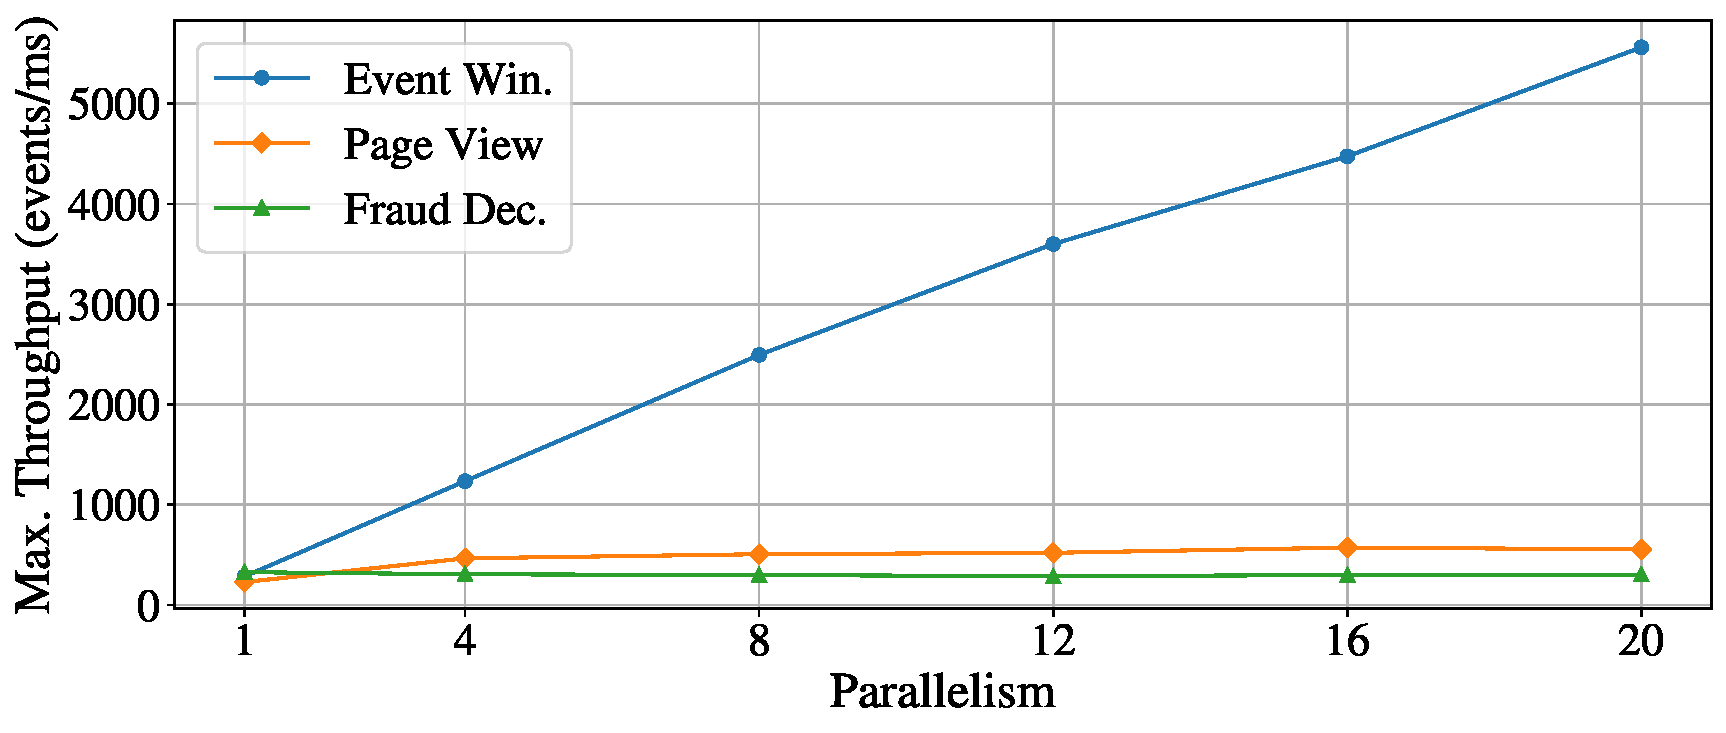
\includegraphics[width=0.8\columnwidth]{figures/dgs/flink_max_throughput_scaleup}

  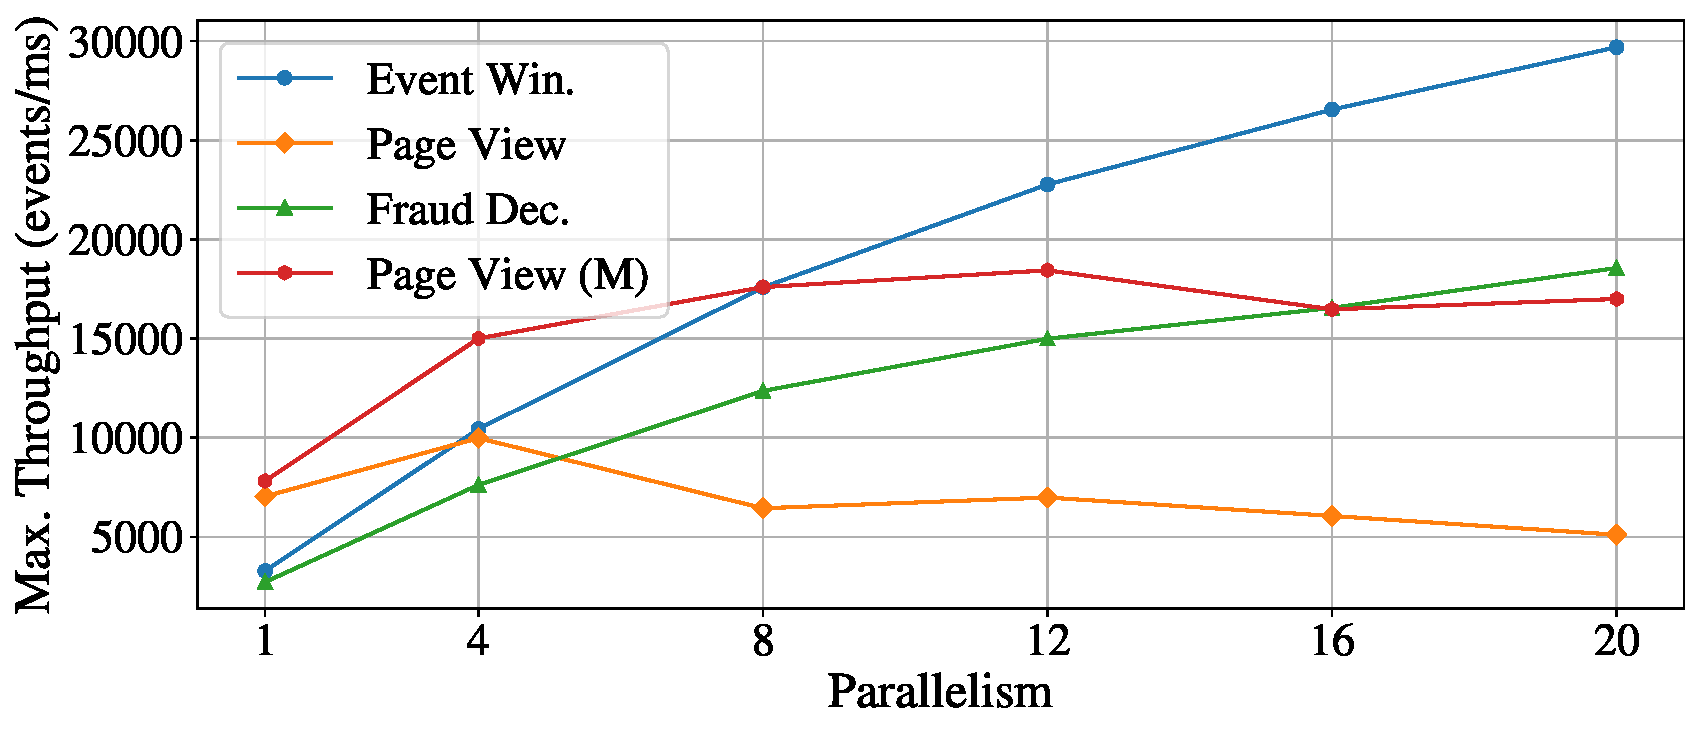
\includegraphics[width=0.8\columnwidth]{figures/dgs/timely_max_throughput_scaleup}
  \caption{
  Flink (top) and Timely (bottom) maximum throughput increase with increasing parallel nodes for the three applications that require synchronization.
  For the page-view example in Timely, two implementations are shown: Page View uses automatic
  parallelism while Page View (M) is the manual parallel implementation
  in \Cref{dgs:fig:timely-snippet}.
  }
  \label{dgs:fig:existing-implementations-scaling}
\end{figure}

In this section we investigate how the Flink and Timely APIs can produce scalable parallel implementations for the aforementioned applications.
We iterated on different implementations resulting in a best-effort attempt to achieve good scalability. These implementations are summarized below, and the source code is presented in the extended version of the paper~\cite{flumina-arxiv}.
For each of the implementations, we then ran an experiment where we increased the number of distributed nodes and measured the maximum throughput of the resulting implementation (by increasing the input rate until throughput stabilizes or the system crashes).
The results are shown in \Cref{dgs:fig:existing-implementations-scaling}.

\begin{figure}[t]
  \centering
\begin{verbatim}
updates.broadcast().filter(move |x| {
    x.name == page_partition_fun(NUM_PAGES, worker_index)
});
\end{verbatim}
  \caption{Snippet from the Timely manual (M) implementation of the page-view join example, satisfying \textbf{PIP1} and \textbf{PIP3} but not \textbf{PIP2}.
}
\label{dgs:fig:timely-snippet}
\end{figure}

\paragraph{Event-based windowing.}
Flink's API supports a \texttt{broadcast} construct that can send barrier events to all parallel instances of the implementation, therefore being able to scale with an increasing parallel input load.
Note that Flink does not guarantee that the broadcast messages are synchronized with the other stream events, and therefore the user-written code has to ensure that it processes them in order.
By transforming these barriers to Flink watermarks that indicate window boundaries, we can then aggregate values of each window in parallel, and finally merge all windows to get the global aggregate.
Similarly, Timely includes a \texttt{broadcast} operator on streams, which sends all barrier events to all parallel instances;
then the \texttt{reclock} operator is used to match values with corresponding barriers and aggregate them.
Both the Flink and Timely implementations scale because the values are much more frequent than barriers, i.e., a barrier every 10K events, and are processed in a distributed manner.

\paragraph{Page-view join.}
The input of this application allows for data parallelism across keys, in this case websites, but also for the same key since some keys receive most of the events.
First, for both Flink and Timely, we implemented this application using a standard keyed join, ensuring that the resulting implementation will be parallel with respect to keys.
As shown by the scalability evaluation, this does not scale to beyond 4 nodes in the case that there are a small number of keys receiving most or all of the events.

We wanted to investigate whether it was possible to go beyond the automatic implementations and scale throughput for events \emph{of the same key}.
To study this, we provide a ``manual'' (M) implementation in Timely (\Cref{dgs:fig:timely-snippet} and \Cref{dgs:fig:existing-implementations-scaling}, bottom). Here, we broadcast \emph{update-page-info} events, then filter to only those relevant to each node, i.e. corresponding to \emph{page-view}s that it is responsible for processing. A similar implementation would be possible in Flink. Unfortunately, our implementation sacrifices \textbf{PIP2}, i.e., the assignment of events to parallel instances
becomes part of the application logic---there are explicit references to the physical partitioning of input streams
(\texttt{page\_partition\_fun}) and the the worker that processes each stream (\texttt{worker\_index}).
Additionally, the implementation broadcasts \emph{all} update events to \emph{all} sharded nodes (not just the ones that are responsible for them), introducing a linear synchronization overhead with the increase of the number of nodes.
An alternative choice would have been to not only broadcast events, but also keep state for \emph{every} page at every sharded replica: this would satisfy \textbf{PIP2} because nodes no longer need to be aware of which events they process, but it does not avoid the broadcasting issue and thus we would expect performance overheads.
Overall, we observe inability to automatically scale this application without sacrificing platform independence in both Flink and Timely.

\paragraph{Fraud detection.}
The standard dataflow streaming API cannot support cross-instance synchronization, and therefore we can only develop a sequential implementation of this application using Flink's API.
Timely offers a more expressive API with \emph{iterative} computation, and this allows for an automatically scaling implementation: after aggregating local state to globally updated the learning model, we have a cyclic loop which then sends the state back to all the nodes to process further events.
The results show that this implementation scales almost as well as the event-based window.
This effectively demonstrates the value of iterative computation in machine learning and complex stateful workflows.

\begin{takeaway}
\textbf{Take-away (Q1):}
The streaming APIs of Flink and Timely cannot automatically produce implementations that scale throughput for all applications that have synchronization requirements without sacrificing platform independence.
\end{takeaway}

\begin{figure}[t]
    \centering
    \begin{subfigure}[b]{0.48\columnwidth}
      \centering
      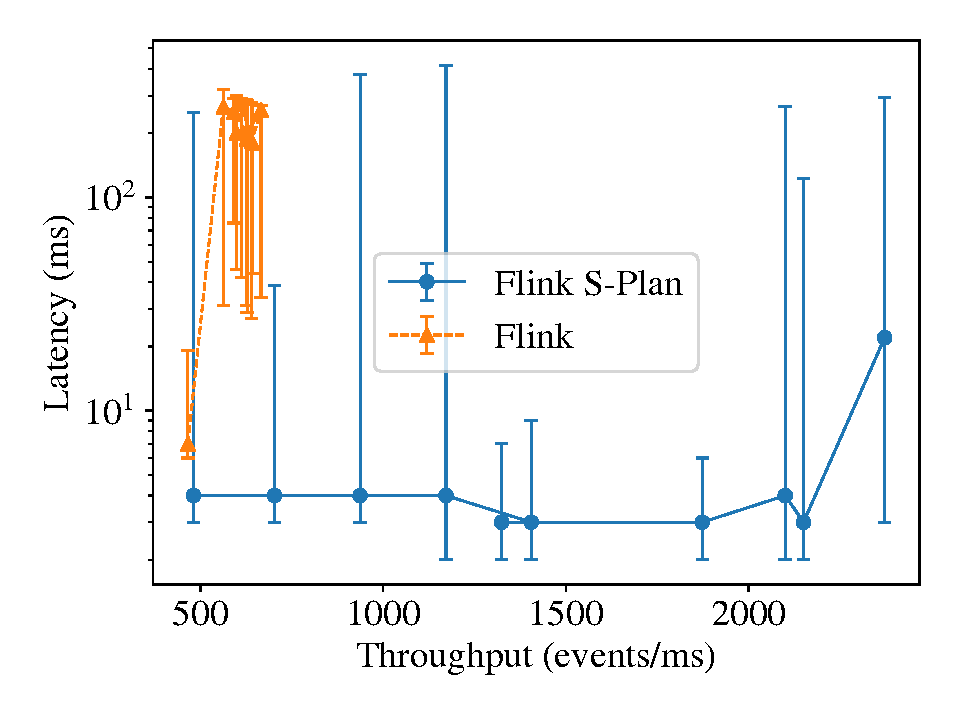
\includegraphics[width=\textwidth]{figures/dgs/pageview-flink-splan.pdf}
      \caption{Page-view join.}
      \label{dgs:fig:synchronization-plan-page-view-join-throughput}
    \end{subfigure}
    ~
    \begin{subfigure}[b]{0.48\columnwidth}
      \centering
      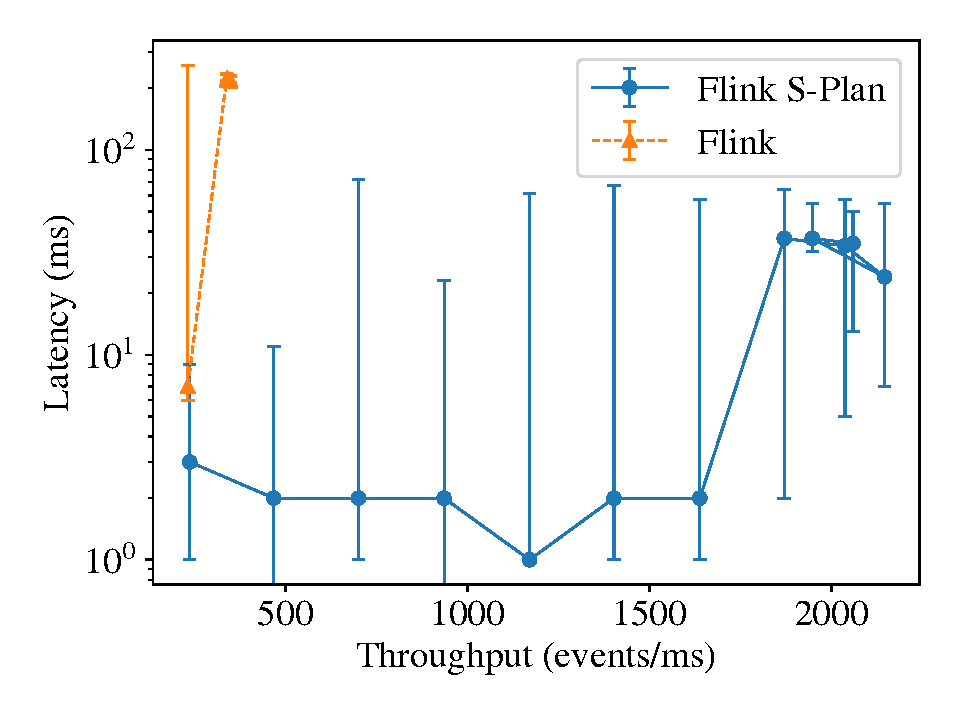
\includegraphics[width=\textwidth]{figures/dgs/frauds-flink-splan.pdf}
      \caption{Fraud detection.}
      \label{dgs:fig:synchronization-plan-fraud-detection-throughput}
    \end{subfigure}
    \caption{
      Throughput (x-axis) and 10th, 50th, 90th percentile latencies on the y-axis for increasing input rates (from left to right) and 12 parallel nodes. Flink (\textcolor{Orange}{orange}) is the parallel implementation produced automatically, and Flink S-Plan (\textcolor{NavyBlue}{blue}) is the synchronization plan implementation.
      }
    \label{dgs:fig:synchronization-plan-throughputs-flink}
\end{figure}

\subsection{Manual synchronization}
\label{dgs:ssec:performance-evaluation}

\begin{figure}[t]
  \centering
% final var invertedUserIds = FlinkHashInverter.getMapping(conf.getTotalUsers());
% updateStream.keyBy(update -> invertedUserIds.get(update.getUserId()))
%         .connect(pageViewStream.keyBy(pv -> invertedUserIds.get(pv.getUserId())))
%         .process(new PageViewProcessParallel(conf.getPageViewParallelism()))
%         .setParallelism(conf.getTotalUsers())
%         // ...
  \begin{minipage}{0.9\textwidth}
  \begin{lstlisting}[language=Java,basicstyle=\small\ttfamily,commentstyle=\scriptsize\ttfamily,morekeywords={var}]
public Integer joinChild(
    final int subtaskId,
    final Integer state
) {
    final int parentId = subtaskId / pageViewParallelism;
    final int childId = subtaskId % pageViewParallelism;
    joinSemaphores.get(parentId).get(childId).release();
    forkSemaphores.get(parentId).get(childId)
        .acquireUninterruptibly();
    return zipCode.get(parentId);
}
  \end{lstlisting}
  \end{minipage}
  \caption{Snippet from the implementation of the manual synchronization \texttt{join} in Flink. This implementation does not satisfy \textbf{PIP1--3}.}
  \label{dgs:fig:flink-snippet}
\end{figure}

\noindent
To address Q2, we next investigate whether synchronization, implemented manually and possibly sacrificing \textbf{PIP1--3}, can offer concrete throughput speedups.
We focus this implementation in Flink, and consider the two applications that Flink cannot produce parallel implementations for, namely \emph{page-view join} and \emph{fraud detection}. We write a DGS program for these applications and we use our generation framework to produce a synchronization plan for a specific parallelism level (12 nodes). We then manually implement the communication pattern for these synchronization plans in Flink, and we measure their throughput and latency compared to the parallel implementations that the systems produced in \Cref{dgs:ssec:eval-existing-implementations}. The results for both applications are shown in \Cref{dgs:fig:synchronization-plan-throughputs-flink}. Flink does not achieve adequate parallelism and therefore cannot handle the increasing input rate (low throughput and high latency).

\paragraph{Page-view join.}
The synchronization plan that we implement for this application is a forest containing a tree for each key (website) and each of these trees has leaves that process page-view events. Each time an update event needs to be processed for a specific key, the responsible tree is joined, processes the event, and then forks the new state back.

\paragraph{Fraud detection.}
The synchronization plan that we implement for this application is a tree that processes rule events at its root and transactions at all of its leaves. The tree is joined in order to process rules and is then forked back to keep processing transactions.

\paragraph{Implementation in Flink.}
In order to implement the synchronization plans in Flink we need to introduce communication across parallel instances. We accomplish this by using a centralized service that can be accessed by the instances using Java RMI. Synchronization between a parent and its children happens using two sets of semaphores, $J$ and $F$.
A child releases its $J$ semaphore and acquires its $F$ semaphore when it is ready to join, and a parent acquires its children's $J$ semaphores, performs the event processing, and then releases their $F$ semaphores (\Cref{dgs:fig:flink-snippet}).
This implementation of manual synchronization
sacrifices all three platform independence principles \textbf{PIP1--3}.
For \textbf{PIP1} and \textbf{PIP2}, it refers explicitly to the number of parallel instances and the partitioning (\texttt{pageViewParallelism}, \texttt{subtaskId}, etc.).
For \textbf{PIP3}, it is not API-compliant because it uses an external service (semaphores) to implement synchronization, whereas Flink's documentation requires that operators lack side effects.
This requirement is imposed because, among other considerations, the use of semaphores might cause the program to fail in cases where
work is interrupted and/or repeated after a node failure.
The full code for the Flink implementation can be found in the extended version of the paper~\cite{flumina-arxiv}.

\begin{takeaway}
\textbf{Take-away (Q2):}
Synchronization plans achieve higher throughputs (4-8x for 12 parallel nodes) over the automatic parallel implementations produced by Flink's API.
\end{takeaway}

\subsection{Implementation in Flumina}
\label{dgs:ssec:eval-prototype-performance}

\begin{figure}[t]
  \centering
  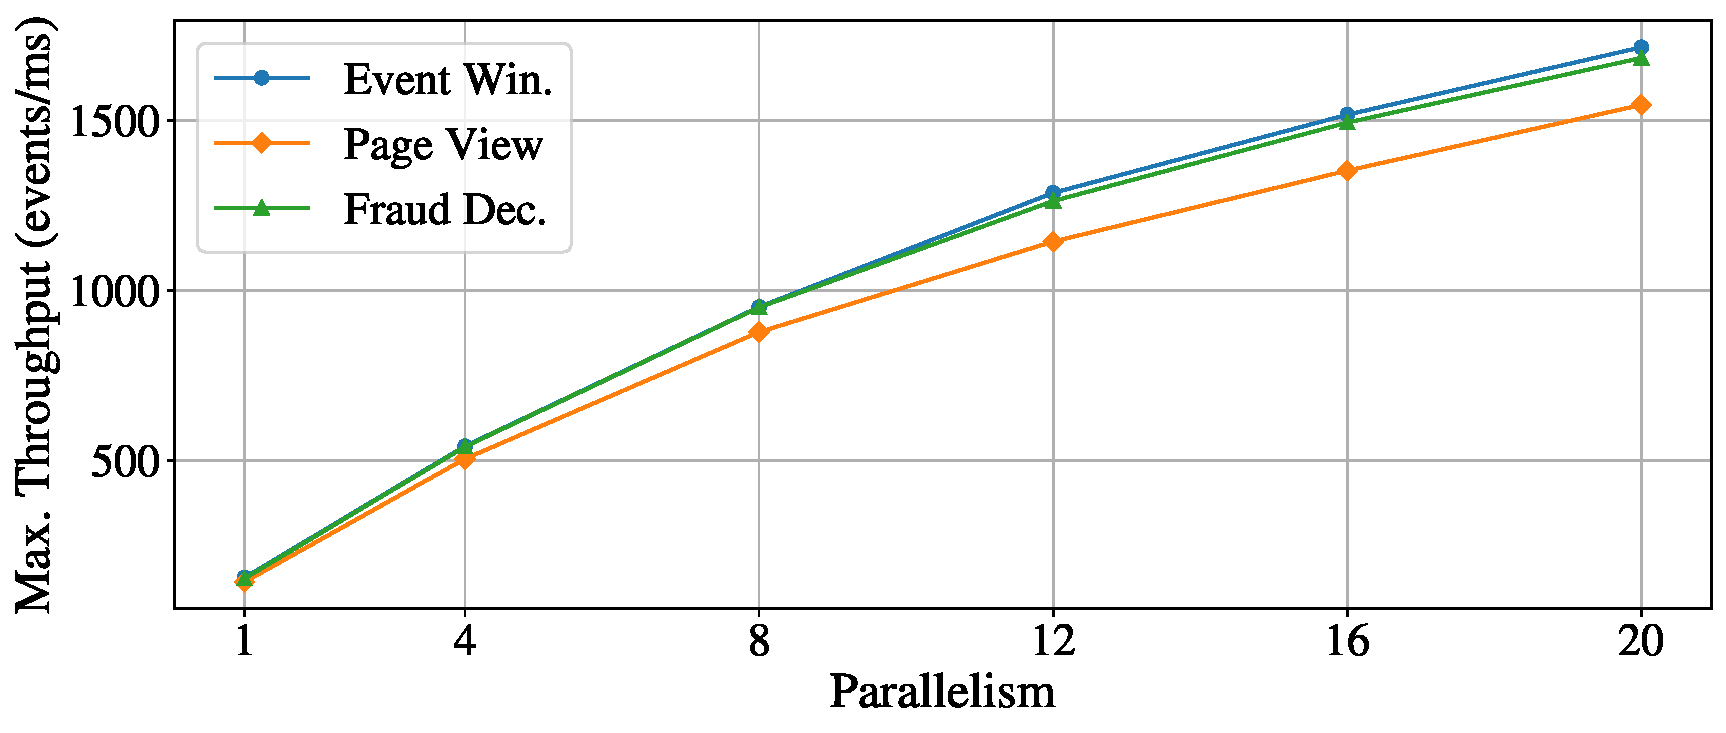
\includegraphics[width=0.8\columnwidth]{figures/dgs/flumina_max_throughput_scaleup.pdf}

  \caption{Flumina (DGS) maximum throughput increase with increasing parallel nodes for the three applications.
  }
  \label{dgs:fig:flumina-scaling}
\end{figure}

To answer Q3, we implement Flumina,
a prototype of our end-to-end framework that can automatically achieve parallelism given a DGS program.
Flumina receives a DGS program written in Erlang,
uses the generation framework that was described in \Cref{dgs:sec:dist-impl} to generate a correct and efficient synchronization plan,
and then implements the plan according to the description in \Cref{dgs:ssec:runtime}.
We implemented all three applications (source code in extended version~\cite{flumina-arxiv})
in Flumina, and measured maximum throughput increase with the addition of parallel nodes
(\Cref{dgs:fig:flumina-scaling}).

\begin{figure}[t]
  \normalsize
  \begin{center}
    \setlength{\tabcolsep}{3pt}
    \renewcommand{\arraystretch}{1.5}
    \begin{tabular}{l | F | T | O | F F | T T | O | F F | T | O}
		& \multicolumn{3}{c|}{Event window} & \multicolumn{5}{c|}{Page-view join} & \multicolumn{4}{c}{Fraud detection} \\
    \hline
    Development tradeoff
     & F & TD & DGS & F & FM & TD & TDM & DGS & F & FM & TD & DGS \\
    \hline
    \textbf{(PIP1)}
  Parallelism independence
		& \cmark & \cmark & \cmark
		& \cmark & \xmark & \cmark & \cmark & \cmark
		& \cmark & \xmark & \cmark & \cmark \\
	\textbf{(PIP2)}
  Partition independence
		& \cmark & \cmark & \cmark
		& \cmark & \xmark & \cmark & \xmark & \cmark
		& \cmark & \xmark & \cmark & \cmark \\
    \textbf{(PIP3)}
  API compliance
		& \cmark & \cmark & \cmark
		& \cmark & \xmark & \cmark & \cmark & \cmark
		& \cmark & \xmark & \cmark & \cmark \\
  Scaling
		& 10x & 8x & 8x
		& 2x & 9x & 1x & 2x & 8x
		& 1x & 9x & 6x & 8x \\
    \end{tabular}

    \phantom{LaTeX is incapable of changing the space in between figure and caption in a sane way.}
  \end{center}
\caption{
Development tradeoffs for each program,
together with throughput scaling for 12 nodes,
in Flink (F), Flink with manual synchronization (FM),
Timely (TD), Timely with manual partitioning (TDM), and our system (DGS).
}
\label{dgs:tab:developer-tradeoffs}
\end{figure}

\paragraph{Event-based windowing and fraud detection.}
The DGS program for event-based windowing contains: (i) a sequential update function that adds incoming value events to the state, and outputs the value of the state when processing a barrier event, (ii) a dependence relation that indicates that all events depend on barrier events, and (iii) a \fl{fork} that splits the current state in half, together with a \fl{join} that adds two states to aggregate them. The DGS program for fraud detection is the same with the addition that the  \fl{fork} also duplicates the sum of the previous transaction and last rule modulo 1000.

\paragraph{Page-view join.}
In addition to the sequential update function, the program indicates that events referring to different keys are independent, and that page-view events of the same key are also independent. The \fl{fork} and \fl{join} are very similar to the ones in \Cref{dgs:fig:key-value-store} and just separate the state with respect to the keys.

\begin{takeaway}
\textbf{Take-away (Q3):}
Across all three examples,
Flumina produces parallel implementations that scale throughput without sacrificing platform independence.
\end{takeaway}

\subsection{Summary: development tradeoffs}
\label{dgs:ssec:eval-development-tradeoffs}

Finally, regarding Q4,
\Cref{dgs:tab:developer-tradeoffs} shows all the tradeoffs that need to be made for each of the programs in this section together with the throughput increase for 12 nodes.
Note that throughput scaling comparison is only relevant for the same system (each of which is denoted with a different color) and not across systems due to differing sequential baselines.
Of all the implementations in \Cref{dgs:ssec:eval-existing-implementations}, the Timely manual page-view example sacrifices \textbf{PIP2}.
The manually synchronizing Flink implementations in \Cref{dgs:ssec:performance-evaluation} show good throughput scaling at the cost of \textbf{PIP1--3}.

\begin{takeaway}
\textbf{Take-away (Q4):}
Of the three APIs studied,
only DGS can achieve scalable implementations across
all examples without sacrificing either parallelism independence, partition independence, or API compliance.
\end{takeaway}


\section{Case Studies}
\label{dgs:appendix:case-studies}

In the next couple of subsections, we evaluate if DGS can be used for realistic application workloads.
We consider the following questions:
\begin{enumerate}
    \item How does the performance of Flumina compare with handcrafted implementations?
    \item What is the additional programming effort necessary to achieve automatic parallelization when using the DGS programming model?
\end{enumerate}

To evaluate these questions we describe two case studies on applications taken from the literature that have existing high-performance implementations for comparison. The first is a state-of-the-art algorithm for statistical outlier detection, and the second is a smart home power prediction task from the DEBS Grand Challenge competition.
For question (1),
the two case studies are posed in the literature targetting different performance metrics: throughput scalability for outlier detection and latency for the smart home task.
We are able to achieve performance comparable to the existing handcrafted implementations in both cases with respect to the targetted metric.
For question (2), this performance is achieved while putting minimal additional effort into parallelization: compared to 200-700 LoC for the sequential task, writing the fork and join primitives requires only an additional 50-60 LoC.
These results support the feasibility of using DGS for practical workloads, with minimal additional programmer effort to accomplish parallelism.

\subsection{Statistical outlier detection}
\label{dgs:ssec:outlier-detection}

\textsc{Reloaded}~\cite{otey2006fast} is a state-of-the-art distributed
streaming algorithm for outlier detection in mixed attribute
datasets. It is a structurally similar
to the fraud-detection example from the experimental evaluation.
The algorithm assumes a set of input streams that
contain events drawn from the same distribution. Each input stream is
processed independently by a different worker with the goal of
identifying outlier events. Each worker constructs a local model of
the input distribution and uses that to flag some events as potential
outliers. Whenever a user (or some other event) requests the current
outliers, the individual workers merge their states to construct a
global model of the input distribution and use that to flag the
potential outlier events as definitive outliers.
We executed a network
intrusion detection task from the original
paper~\cite{kddcup1999dataset}.
The goal of the task is to distinguish malicious connections from a
streaming dataset of simulated connections on a typical U.S.~Air Force
LAN. Each connection is represented as an input event. In the
experiment we varied the number of nodes from 1-8 and we measured the
execution time speedup. We executed this experiment on a local server
(Intel Xeon Gold 6154, 18 cores @3GHz, 384 GB) with the NS3~\cite{carneiro2010ns3} network simulator
to have comparable network latency with the original paper that used a small local cluster.

\paragraph{Programmability.}
The sequential implementation of the algorithm in DGS consists of approximately 700
lines of Erlang code---most of which is boilerplate to manage the
data structures of the algorithm.
Compared to the sequential implementation, the programming effort to achieve a
parallel implementation is a straightforward pair of \texttt{fork} and \texttt{join} primitives, which amounts to 50~LoC.

\paragraph{Performance.}
DGS and synchronization plans can capture the complex synchronization pattern that was proposed for \textsc{Reloaded}, achieving comparable speedup to that reported in the original paper:
almost linear (7.3$\times$ for 8 nodes), compared to 7.7$\times$ for 8 nodes by the handcrafted C++ cluster evaluation reported in the paper.

\subsection{IoT power prediction}
\label{dgs:ssec:iot-case-study}

The DEBS Grand Challenge is an annual competition to evaluate how
research solutions in distributed event-based systems can perform on
real applications and workloads.  The 2014
challenge~\cite{jerzak2014debs2014, DEBS2014web} involves an IoT task
of power prediction for smart home plugs.  As with the previous case
study, our goal is to see if the performance and programmability of
our model and framework can be used on a task where there are
state-of-the-art results we can compare to.
The problem (query 1 of the challenge) is to predict the load of a
power system in multiple granularities (per plug, per house, per
household) using a combination of real-time and historic data.  We
developed a solution that follows the suggested prediction method,
that involves using a weighted combination of averages from the hour and
historic average loads by the time of day.  This task involves
inherent synchronization: while parallelization is possible at each of
the different granularities, synchronization is then required to bring
together the historic data for future predictions. For example, if
state is parallelized by plug, then state needs to be joined in order
to calculate a historic average load by household.  Our program
is conceptually similar to the map from keys to counters in
\Cref{dgs:sec:prog-model}, where we maintain a map of historical totals
for various keys (plugs, houses, and households).  The challenge input
contains 29GB of synthetic load measurements for 2125 plugs
distributed across 40 houses, during the period of one month.  We
executed our implementation on a subset of 20 of the 40 houses, which
we sped up by a factor of 360 so that the whole experiment took about
2 hours to complete.  To compare with submissions to the challenge
which were evaluated on one node, we ran a parallelized computation on
one server node.
To simulate the network and measure network load, we
then used NS3 \cite{carneiro2010ns3}.

In the state, we maintain a set of maps of recent and historical
averages for house, household, and plug.  Then, we set different
houses, $\tg{house}_k$ (for $k$ between $1$ and $20$) to be
different tags, and we add an end-timeslice event $\tg{\#}$
at the end of every hour.  The dependence relation is that
end-timeslice is dependent on everything (this is when output is
produced), and that $\tg{house}_k$ is dependent on itself for every
$k$, but independent of other houses.  The \emph{fork} function
splits each map by house ID, and the \emph{join} function merges
maps back together.

\paragraph{Programmability.}
In total, the sequential code of our solution amounted to about 200~LoC, and the parallelization primitives (fork, join,
dependence relation) were 60~LoC.  We conclude that the overhead to enable
parallelization is small compared to the sequential code.

\paragraph{Performance.}
Latency varied between $44$ms (10th percentile), $51$ms (median), and
$75$ms (90th), and the average throughput was $104$
events/ms. These results are on par with the ones reported
by that year's grand challenge winner~\cite{mutschler2014predictive}:
$6.9ms$ (10th) $22.5ms$ (median) 41.3 (90th) and $131$ events/ms
throughput.
Note that although the dataset is the same,
the power prediction method used was different in some solutions.  In
this application domain, our optimizer has the advantage of enabling
edge processing: we measure only 362~MB of data sent over the network,
in contrast to the 29~GB of total processed data.

\section{Outtakes}

(Author's note: this material was delegated to the appendix of the original paper and can be found in the extended version~\cite{flumina-arxiv}.)

\subsection{Communication Optimizer}
\label{dgs:appendix:optimizer}

In this section we describe one of the synchronization plan optimizers that we have developed, namely one that is based on a simple
heuristic: it tries to generate a synchronization plan with a
separate worker for each input stream, and then tries to place these
workers in a way that minimizes communication between them.
This optimizer assumes a network of computer nodes and takes as input
estimates of the input rates at each computer node. It searches for an
$P$-valid synchronization plan that maximizes the number of events
that are processed by leaves; since leaves can process events
independently without blocking. The optimizer first uses a greedy
algorithm that generates a graph of implementation tags (where the
edges are between dependent tags) and iteratively removes the implementation
tags with the lowest rate until it ends up with at least two
disconnected components.

\begin{example}
\label{dgs:example:optimization}
For an example optimization run, consider \Cref{dgs:fig:example-configuration},
and suppose that $\tg{r}(2)$ has a rate of 10 and arrives at node $E_0$,
$\tg{r}(1)$, $\tg{i}(1)$ have rates of 15 and 100 respectively and arrive at node $E_1$,
$\tg{i}(2)_a$ has rate 200 and arrives at node $E_2$,
and $\tg{i}(2)_b$ has rate 300 and arrives at node $E_3$.
Since events of different keys are independent, there are
two connected components in the initial graph---one for each
key. The optimizer starts by separating them into two
subtrees. It then recurses on each disconnected component, until there
is no implementation tag left, ending up with the tree structure shown
in \Cref{dgs:fig:example-configuration}. Finally, the optimizer
exhaustively tries to match this implementation tag tree, with a
sequence of forks, in order to produce a valid synchronization plan
annotated with state types, updates, forks, and joins.
This generates the implementation in \Cref{dgs:fig:distr_arch}.
\end{example}

\begin{figure}[t]
  \begin{tikzpicture}[scale=0.7,transform shape,sibling distance=30em, level distance=80pt,
    every node/.style = {shape=rectangle,
      rounded corners,
      draw, align=center},
    level 1/.style = {sibling distance=30em},
    level 2/.style = {sibling distance=13em}]]

    \node (e0) { \TopDNode{$w_1$}{ }
                          {$E_0$}{update -- $\langle$ fork, join $\rangle$} }
      child { \DNode{$w_2$}{$\tg{r}(1), \tg{i}(1)$}{$E_1$}{update}{e1} }
      child { \DNode{$w_3$}{$\tg{r}(2)$}{$E_0$}{update -- $\langle$ fork, join $\rangle$}{e23}
          child { \DNode{$w_4$}{$\tg{i}(2)_a$}{$E_2$}{update}{e2} }
          child { \DNode{$w_5$}{$\tg{i}(2)_b$}{$E_3$}{update}{e3} } };

      %% Make the nodes
      \node (node0) [above=1mm of e0.north west, draw=none] { $E_0$ };
      \node [draw=black!50, fit={(e0) (e23) (node0)}, rounded corners=0] (c0) {};

      \node (node1) [above=1mm of e1.north west, draw=none] { $E_1$ };
      \node [draw=black!50, fit={(e1) (node1)}, rounded corners=0] (c1) {};

      \node (node2) [above=1mm of e2.north west, draw=none] { $E_2$ };
      \node [draw=black!50, fit={(e2) (node2)}, rounded corners=0] (c2) {};

      \node (node3) [above=1mm of e3.north west, draw=none] { $E_3$ };
      \node [draw=black!50, fit={(e3) (node3)}, rounded corners=0] (c3) {};

      %% Input streams

      \coordinate[right=20mm of c0] (d0);
      \coordinate[above=5mm of d0] (dd0);
      \coordinate[above=5mm of c0.east] (dc0);
      \draw [->] (d0) to[left] node[draw=none, auto] {$\tg{r}(2)$, 10} (c0);
      \draw [->] (dc0) to[right] node[draw=none, auto] {$val$} (dd0);

      \coordinate[left=20mm of c1] (d1);
      \coordinate[above=5mm of d1] (dd1);
      \coordinate[above=5mm of c1.west] (dc1);
      \coordinate[below=5mm of d1] (dd2);
      \coordinate[below=5mm of c1.west] (dc2);
      \draw [->] (d1) to[right] node[draw=none, auto] {$\tg{i}(1)$, 100} (c1);
      \draw [->] (dd1) to[right] node[draw=none, auto] {$\tg{r}(1)$, 15} (dc1);
      \draw [->] (dc2) to[left] node[draw=none, auto] {$val$} (dd2);

      \coordinate[left=20mm of c2] (d2);
      \draw [->] (d2) to[left] node[draw=none, auto] {$\tg{i}(2)_a$, 200} (c2);

      \coordinate[right=20mm of c3] (d3);
      \draw [->] (d3) to[right] node[draw=none, auto] {$\tg{i}(2)_b$, 300} (c3);

  \end{tikzpicture}
  \caption{Example synchronization plan generated in \Cref{dgs:example:optimization}.
  The large gray rectangles $E_0$, $E_1$, $E_2$, $E_3$ represent physical nodes
  and the incoming arrows represent input streams and their relative rates.}
  \label{dgs:fig:distr_arch}
\end{figure}

\subsection{Correctness Proof}
\label{dgs:appendix:correctness}

We prove \Cref{dgs:theorem:correctness} and therefore show that our framework is correct according to \Cref{dgs:def:distr-correctness}.
The key assumptions used are:
\begin{enumerate}
\item[(1)] The program is consistent, as defined in \Cref{dgs:ssec:prog-model-correctness}.
\item[(2)] The input streams constitute a valid input instance, as defined in \Cref{dgs:def:valid-input-instance}.
\item[(3)] The synchronization plan that is chosen by the optimizer is valid, as defined in \Cref{dgs:ssec:distributed-configurations}.
\item[(4)] Messages that are sent between two processes in the system arrive in order and are always received. This last assumption is ensured by the Erlang runtime.
\item[(5)] The underlying scheduler is fair, i.e. all processes get scheduled infinitely often.
\end{enumerate}

The proof decomposes the implementation into the mailbox
implementations and the worker implementations, which are both sets of
processes that given a set of input streams produce a set of output
streams. We first show that the mailboxes transform a valid input
instance to a worker input that is correct up to reordering of
independent events. Then we show that given a valid worker input, the
workers processes' collective output is correct.
The second step relies on
\Cref{dgs:thm:consistency-implies-determinism},
from the previous section, as well as
\Cref{dgs:lemma:worker-wire-correspondence}
which ties this to the mailbox implementations,
showing that the implementation produces a valid wire diagram according to the formal semantics of the program $P$.
Given a valid input instance $u$ and a computation program $P$ that contains
in particular a sequential specification \fl{spec: List(Event) -> List(Out)},
we want to show that any implementation $f$ that is produced by our framework is correct according to \Cref{dgs:def:distr-correctness}.

\begin{definition}
For a valid input instance $u$, a worker input $m_u = (m_1, ..., m_N)$
is \emph{valid} with respect to $u$ if $m_i \in \mathrm{reorder}_{D_I}
(\mathrm{filter}(\mathrm{rec}_{w_i}, \mathrm{sort}_O(u))),$ where
$\mathrm{reorder}_{D_I}$ is the set of reorderings that preserve the
order of dependent events,
  $\mathrm{rec}_w(\langle \sigma, t, p\rangle) = \sigma \in \mathrm{atags}(w) \cup w.\mathsf{itags}$
  is a predicate of the messages that each worker $w$ receives,
  and $\mathrm{atags}$ is the set of implementation tags that are handled by a workers ancestors, and is given by $\mathrm{atags}_w = \{ {w'}.\mathsf{itags} : \forall w' \in \mathrm{anc}(w', w)\}$.
\end{definition}

\begin{lemma}
\label{dgs:lemma:mailbox}
Given a valid input instance $u$, any worker input $m$ produced by
the mailbox implementations $(u, m)$ in $f$ is valid with respect to
$u$.
\end{lemma}
\begin{proof}
By induction on the input events of one mailbox and using assumptions
(2)-(5).
\end{proof}

Each worker $w$ runs the update function on each event $e = \langle
\sigma, t, p\rangle$ on its stream that it is responsible for $\sigma
\in w.\mathsf{itags}$ possibly producing output $\fl{o: List(Out)}$.
For all events in the stream that one of its
ancestors is responsible for, it sends its state to its parent worker
and waits until it receives an updated one.
The following key lemma states that this corresponds to a particular
wire diagram in the semantics of the program.

\begin{lemma}
\label{dgs:lemma:worker-wire-correspondence}
Let $m$ be the worker input to $f$ for program $P$
on input \fl{u},
and let $\fl{o}_i: \fl{List(Out)}$ be the stream of output events
produced by worker $i$ on input $m_i$.
Then there exists \fl{v: List(Out)}
such that $\fl{inter}(\fl{v}, \fl{o}_1, \fl{o}_2, \ldots, \fl{o}_N)$
and $(\fl{u}, \fl{v}) \in \sem{S}$.
\end{lemma}
\begin{proof}
By induction on the worker input and using assumption (3), in particular
validity condition (V1),
we first show that the worker input corresponds to a wire diagram,
in particular we show that
$\semantics{\fl{State_0}}{\fl{true}}{\fl{s}}{\fl{u}'}{\fl{s'}}{\fl{v}}$
where \fl{v} is an interleaving of $\fl{o}_1, \ldots, \fl{o}_N$
and $\fl{u}'$ is \emph{any} interleaving of the events
$\fl{u}'_i$
processed by each mailbox, namely
$\mathrm{filter}(\mathrm{rec}_{w_i}, {w_i}.\mathsf{itags})$.
Applying \Cref{dgs:lemma:mailbox},
\fl{u} is one possible interleaving of the events $\fl{u}'_i$
and hence we conclude that
$\semantics{\fl{State_0}}{\fl{true}}{\fl{s}}{\fl{u}}{\fl{s'}}{\fl{v}}$,
thus
$(\fl{u}, \fl{v}) \in \sem{S}$.
\end{proof}

Combining \Cref{dgs:lemma:worker-wire-correspondence}
and \Cref{dgs:thm:consistency-implies-determinism} then yields the end-to-end correctness theorem \Cref{dgs:theorem:correctness}.

\subsection{Flumina System Details}
\label{dgs:appendix:flumina-impl}

\paragraph{Flumina synchronization latency}
\label{dgs:ssec:latency-eval}
We also conducted an experiment to evaluate the latency of synchronization plans. We studied three factors that affect latency: (i) the depth of the synchronization plan, (ii) the rate of events that are processed at non-leaf nodes of the plan, and (iii) the heartbeat rate. We ran the event-based windowing application with various configurations and the results are shown in \Cref{dgs:fig:synchronization-overhead}.
\begin{figure}[t]
    \centering
    \begin{subfigure}[t]{0.45\columnwidth}
      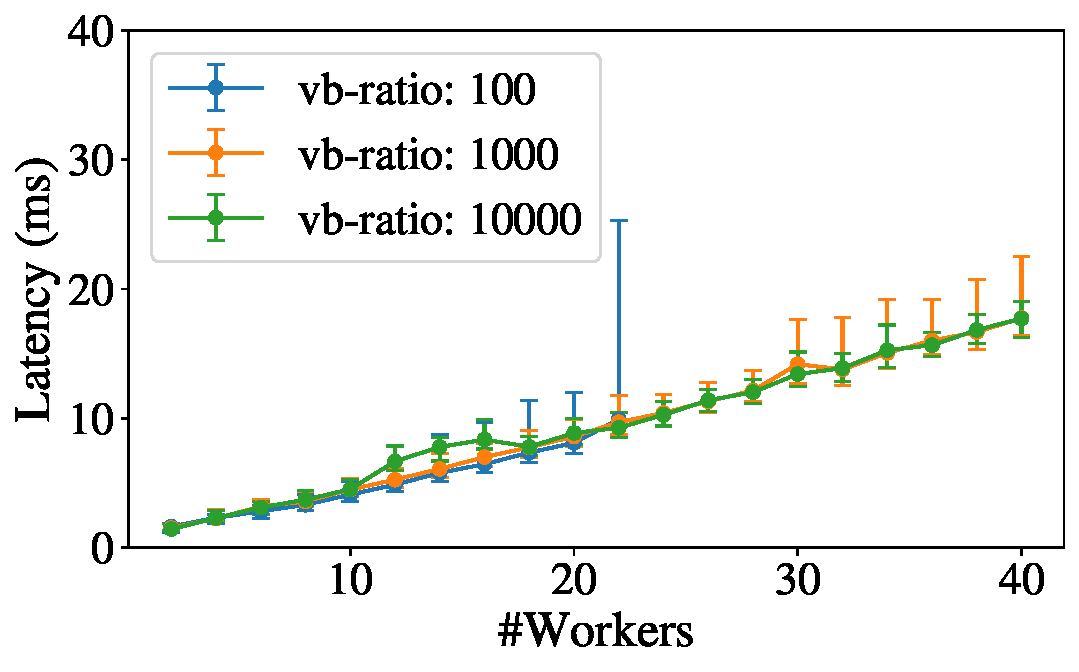
\includegraphics[width=\textwidth]{figures/dgs/synchronization_cost_ratios_nodes}
    \end{subfigure}
    \begin{subfigure}[t]{0.45\columnwidth}
      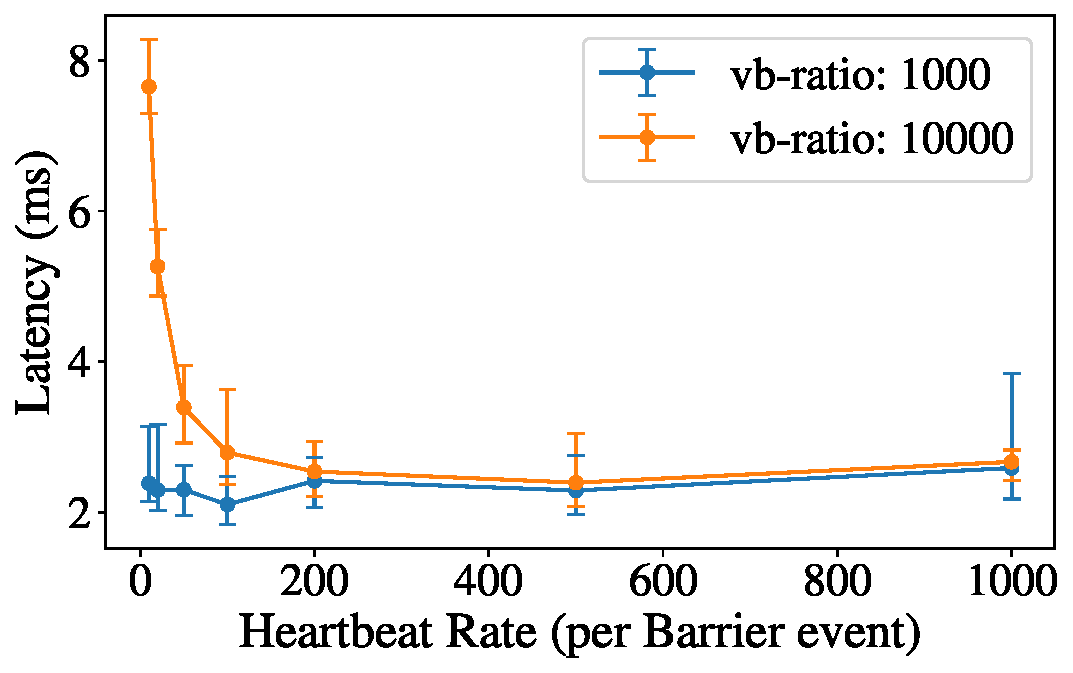
\includegraphics[width=\textwidth]{figures/dgs/synchronization_cost_heartbeats_ratios}
    \end{subfigure}
    \caption{
    Flumina latency (10/50/90 percentile) on the event-based windowing application for various configurations:
    Synchronization impact on latency (10/50/90 percentile) for various configurations:
    \textbf{(a)}
    Varying ratios of value to barrier events (different lines) and number of parallel nodes (x-axis). Heartbeat ratio is 1/100 the vb-ratio. The blue line stops after 22 workers.
    \textbf{(b)} Varying ratios of value to barrier events (different lines) and heartbeat rates (x-axis). Number of parallel nodes is fixed to 5.
      }
    \label{dgs:fig:synchronization-overhead}
\end{figure}
Latency increases linearly with
the number of workers, since the more workers there are, the more
messages have to be exchanged when a barrier event occurs. Note that
the latencies are higher for lower vb-ratios since every time a barrier
event occurs, all of the nodes need to synchronize. In particular, the
system cannot handle beyond 22 workers for vb-ratio of 100 (i.e. 100
forks-joins of the whole synchronization plan per second). On the right,
we see that if the heartbeat rate is too low latency increases since worker mailboxes cannot release events quickly and therefore get filled up, only releasing events in big batches whenever a barrier occurs.

\paragraph{State checkpoints}
Flumina provides a simple yet effective state checkpointing mechanism
for resuming a computation in case of faults.
In contrast to other distributed stream processing systems, where the
main challenge for checkpointing state is the acquisition of
consistent distributed
snapshots~\cite{Naiad2013,Flink2017},
performing a state checkpoint is straightforward when the root
node has joined the states of its descendants.
The joined state at that point in time (which corresponds to
the timestamp of the message that triggered the join request) is a
consistent snapshot of the distributed state of the system, and
therefore we get a non pausing snapshot acquiring mechanism for free.
We have exploited this property of Flumina to implement a programmable
checkpoint mechanism that is given to the system as an option when
initializing worker processes. The checkpoint mechanism can be
instantiated to save a snapshot of the state every time the state is
joined on the root node, or less frequently, depending on an arbitrary
user defined predicate. We implemented a checkpoint mechanism that
produces a checkpoint every time the root node joins its children
states.

\section{Discussion}
\label{dgs:sec:conclusion}

There are a wealth of problems that we left open in this work.
One problem that is not yet adequately explored in our framework is optimization:
given a DGS program, how to select a valid synchronization plan which is most efficient according to a desired cost metric.
Traditional optimization algorithms for stream processing systems cannot be directly applied to
the complex tree structure of synchronization plans.
There are also possibilities for
dynamic optimization, in which the synchronization plan is modified online in response to profiling data from the system.
Besides optimization, the implementation of synchronization plans needs to address a plethora of systems related issues, such as (i) the efficient management and communication of forked state in a distributed environment, (ii) execution guarantees in the presence of faults, and (iii) supporting performance optimizations such as batching and backpressure.

I find the core programming model of \Cref{dgs:sec:prog-model} to be extremely promising and exciting. One thing we have wondered is whether it can be applied outside of the context of streaming, more generally for distributed programming. Related work in consistent replicated distributed systems
(e.g. RedBlue consistency~\cite{li2012making};
MixT~\cite{milano2018mixt} and Gallifrey~\cite{milano2019tour};
and Hamband~\cite{houshmand2022hamband})
suggests a starting point.
